\documentclass[12pt]{puthesis}
%\documentclass[12pt,lot, lof, singlespace]{puthesis}
%\newcommand{\printmode}{}

% Front page materials
\title{Spectroscopic Characterization of New Er$^{3+}$ Host Crystals for Quantum Network Applications}
\submitted{May 2020}  
\copyrightyear{May 2020}  
\author{Henry Allen Ando}
\adviser{Professor Jeff D. Thompson}  
\department{Physics}

% Import packages
\usepackage{graphicx}
\usepackage{verbatim}
\usepackage{multirow}
\usepackage{longtable}
\usepackage{booktabs}
\usepackage{amsmath}
\usepackage{amssymb}
\usepackage{graphicx}
\usepackage{caption}
\usepackage[table,xcdraw]{xcolor}
\usepackage{tikz}
\usepackage{siunitx}
\usepackage{tabularx}
\usepackage{booktabs}
\usepackage[english]{babel}
\usepackage[autostyle, english = american]{csquotes}
\usepackage{siunitx}
\usepackage{float}
\usepackage{array}
\usepackage{paralist}
\usepackage{cite} 
\usepackage{multicol} 
\usepackage{wrapfig}
\usepackage{adjustbox}
\usepackage{physics}
\usepackage{rotating}
\setlength{\LTcapwidth}{\textwidth}

% Set page geometry options
\usepackage[colorlinks=true,linkcolor=black,citecolor=blue]{hyperref}
\usepackage[margin=1in]{geometry}
\setlength\parindent{28pt}
\usepackage{setspace}
\onehalfspacing

% Define functions
\newcommand{\erbium}[1][ ]{Er$^{3+}$#1}
\newcommand{\YSO}[1][ ]{Y$_{2}$SiO$_{5}$#1}
\newcommand{\ErYSO}[1][ ]{Er$^{3+}$:Y$_{2}$SiO$_{5}$#1}
\newcommand{\TiO}[1][ ]{TiO$_{2}$#1}
\newcommand{\MgO}[1][ ]{MgO#1}
\newcommand{\MgO2}[1][ ]{MgO$^{2+}$#1}
\newcommand{\O2}[1][ ]{O$^{2-}$#1}
\newcommand{\supercite}[1]{$^{\text{\cite{#1}}}$}
\graphicspath{{Figures/}}
\newcommand{\notetoself}[1]{\textcolor{red}{#1}}
\newcommand{\wn}[1][ ]{cm$^{-1}$#1}

% Tweak float placements
\renewcommand{\topfraction}{0.85}  % max fraction of floats at top
\renewcommand{\bottomfraction}{0.6}  % max fraction of floats at bottom
\setcounter{topnumber}{2}
\setcounter{bottomnumber}{2}
\setcounter{totalnumber}{4}  % 2 may work better
\setcounter{dbltopnumber}{2}  % for 2-column pages
\renewcommand{\dbltopfraction}{0.66}  % fit big float above 2-col. text
\renewcommand{\textfraction}{0.15}  % allow minimal text w. figs
\renewcommand{\floatpagefraction}{0.66}	 % require fuller float pages
\renewcommand{\dblfloatpagefraction}{0.66}  % require fuller float pages

% Printed vs. online formatting
\ifdefined\printmode
\usepackage{url}
\else
\ifdefined\proquestmode
\hypersetup{bookmarksnumbered}
\makeatletter
\hypersetup{pdftitle=\@title,pdfauthor=\@author}
\makeatother
\else
\hypersetup{colorlinks,bookmarksnumbered}
\makeatletter
\hypersetup{pdftitle=\@title,pdfauthor=\@author}
\makeatother
\fi % proquest or online formatting
\fi % printed or online formatting

% Enable or disable front matter
\ifodd 1
\renewcommand*{\makecopyrightpage}{}
\renewcommand*{\makeabstract}{}
% \renewcommand{\maketitlepage}{}
\else
\abstract{Large-scale quantum networks will require reliable single-photon sources for distributing entanglement over long distances. The \erbium ion is a good candidate for this purpose as it has an optically accessible transition at 1550 nm, the so-called ``telecom'' wavelength at which light propagates through optical fibers with minimal loss. However, this transition is electric-dipole forbidden and thus spontaneous emission from it is slow (around 100 Hz).
Such a bandwidth constraint would be crippling in a real photonic quantum system. The Thompson lab has bulk-doped \erbium ions into \YSO and then coupled them to silicon nanophotonic cavities, enabling the observation of single photon emissions and enhancing the spontaneous emission rate by a factor of 600 through the Purcell effect \cite{Dibos2017}.
However, the bulk-doped \ErYSO has two downsides. One is that \YSO has strong nuclear spins which limit the  $T_{1}$ and $T_{2}$ spin coherence times of the \erbium ions. The other is that the lower bound on the density of \erbium possible through the bulk-doping process is still too high for individual \erbium ions to be addressed optically.
These issues have motivated a search for new host crystals which can be doped with \erbium through ion implantation, hopefully resulting in substantially lower concentrations of \erbium ions than would be possible through bulk doping. In this work, we characterize the spectral properties of \erbium implanted in various new host crystals, and discuss new techniques for improving the resolution of future such measurements.}
\acknowledgements{Acknowledgements will go here.}
\dedication{To my parents.}
\fi

%%%%%%%%%%%%%%%%%%%%%%%%%%%%%%%%%%%%%%%%%%%%%%%%%%%%%%%%%%%%

\begin{document}
\makefrontmatter

%%%%%%%%%%%%%%%%%%%%%%%%%%%%%%%%%%%%%%%%%%%%%%%%%%%%%%%%%%%%

\chapter{Introduction}
\section{A Brief History of Quantum Computing}
\label{sec:brief-hist-quant}

Humans have studied the stars since the beginning of recorded history, and the ancient Greeks were already wondering about the building blocks of reality. Thus, relative to astrophysics or particle physics, quantum computing could be considered a fairly new field. Quantum computers were originally proposed in the early 1980's as a means of simulating quantum many-body problems that are intractible on classical computers \cite{Feynman1982}. The groundwork of the theory was originally laid out largely by Benioff and Feynman \cite{Benioff1980,Feynman1982}. Toffoli created the first set of universal, reversible quantum logic gates \cite{Toffoli1980}. The no-cloning theorem, which states that \textit{qubits}\footnote{ Qubits, short for quantum bits, are two-element quantum spinors. Photon polarization and electron spin are common examples. A quantum computer has several qubits and performs unitary gates on them analogously } cannot be copied, was proved by Wootters and Zurek \cite{Wootters1982}. In 1985, Deutsch proposed the first model for a universal quantum computer \cite{Deutsch1985}.

As the theory developed throughout the 1990's, theorists began to discover problems whose computational complexity could be vastly reduced on quantum computers. The first example, the Deutsch-Josza algorithm for determining whether a black-box function is either constant or balanced, is of little practical use but inspired many later such algorithms \cite{Deutsch1992}. Another important such discovery is Grover's algorithm for database searches, which offers a quadratic speedup over the classical version \cite{Grover1996}. Perhaps the most important of these discoveries, however, was Shor's algorithm (proposed in 1994), which provides an exponential speedup on the discrete logarithm and large integer factorization problems \cite{Shor1994}. Since most modern telecommunications\footnote{ and thus most of the internet.} are encrypted using RSA encryption schemes which rely on the difficulty of factorizing products of large prime numbers, a real quantum computer capable of running Shor's algorithm would instantly break the encryption on almost the entire internet. It was this discovery which catapulted the field of quantum computing from being an interesting physics experiment to a global arms race involving the governments of the United States and China,\footnote{ among others.} as well as tech companies such as Google, IBM, and Microsoft. 

But while quantum computers threaten to break classical factorization-based encryption methods, they create in exchange the possibility for physically un-interceptible encrypted communication. The oldest and most famous of these so-called \emph{quantum cryptography} schemes is the BB84 protocol for quantum key distribution. This protocol, which encodes information in the polarization states of photons, enables one party to send a private key to another in such a way that any attempt to intercept the message would be detectable to the receiver \cite{Bennett2014,Shor2000}. Another uniquely quantum communication procedure is \emph{teleportation}. In quantum teleportation, a qubit is transmitted from one party to another instantaneously across arbitrarily large distances. This doesn't violate the lightspeed limit for the transfer of information, because a qubit isn't information, and because the protocol requires a classical bit to be exchanged beforehand anyway \cite{Bennett1993}. 

% \notetoself{Here is a potential spot to talk about error correction. However, I'm not sure it's worth the space/time. For the moment, I'll leave only this reminder.}

So far, the theory of quantum algorithms and protocols has ranged far ahead of the ability to physically implement them. Over the years, a few broad classes of physical quantum computers have emerged as the most studied, each for slightly different types of problems. A few of these classes are:
\newcommand{\listheader}[1]{\textbf{#1}}
\begin{itemize}
  
\item \listheader{Trapped ion quantum computers} use the electronic spins of ions trapped in an optical lattice as the qubit \cite{Cirac1995}. Alternatively, trapped neutral atoms can be used, with nuclear spins as the qubits \notetoself{[?]}. The dipole-dipole interactions between adjacent particles can be tuned to perform two-qubit gates, thus making atom trap quantum computers a viable platform for a universal quantum computer \notetoself{[?]}.
  
\item \listheader{Nuclear magnetic resonance (NMR) quantum computers} use the nuclear spins of atoms or molecules dissolved in solution as the qubit \cite{Cory1997}. Unfortunately, it was shown after a few seemingly successful bulk NMR demonstrations that no entanglement had actually occurred in these experiments, and that entangelement is a necessary part of most important quantum algorithms \cite{Braunstein1999,Linden2001}. It was also hard to scale these computers, as each extra qubit required the synthesis of a new molecule. However, the legacy of NMR computers lives on, as many current quantum computing schemes (see the next list item) make use of the main ideas of NMR computers.
  
\item \listheader{Point defects in solid state hosts} such as rare earth ions or nitrogen-vacancy (NV) centers in crystals are in some sense descendents of NMR-based quantum computing paradigms \notetoself{[?]}. In these systems, the spin states of valence electrons serve as qubits. Light-matter interfaces can be achieved by coupling these atoms with photons at the same energy as an optical transition in the qubit atom \notetoself{[?]}. 

\item \listheader{Linear optical quantum computers} use the polarization states of photons as qubits \cite{Knill2001}. The main advantage of this paradigm is that it enables easy transfer of qubits over long distance, because the computational qubits can be sent directly over long distances, either through fiber optic cables or through free space telescopes, with no extra conversion step. 
    
\item \listheader{Superconducting circuit quantum computers} use the phase differences across superconducting Josephson junctions as qubits \cite{Nakamura1999}. These types of computers have so far been the largest, with Google claiming to demonstrate \emph{quantum supremacy} (the ability of a quantum computer to solve a problem faster than a classical counterpart) for the first time on a 53-qubit superconducting quantum computer in 2019 \cite{Arute2019}.
  
\end{itemize}

Although superconducting circuit quantum computers have been the most successful so far in terms of implementing complicated quantum algorithms, they are not so useful for quantum networks applications. Linear optical quantum computers are the best suited for working purely with photonic qubits in quantum networks, but without the superior computing power offered by superconducting circuits can only implement fairly simple tasks. Thus, point defects in solid state hosts are a very exciting platform, as they offer the possibility of light-matter interfaces that could marry the power of superconducting circuit computers with the distance allowed by photons. This would enable a variety of exciting quantum technologies, such as quantum cryptography, quantum-enhanced metrology, and modular quantum computing \cite{Monroe2014}.

\section{\erbium in crystals as a technology for quantum networks }
\label{sec:erbium-crystals-as}

Single atoms and atom-like defects in crystals have successfully demonstrated a variety of quantum-network-related tasks. Examples include spin-photon entanglement in quantum dots \cite{Greve2012}, entanglement between trapped atoms and photons \cite{Blinov2004}, teleportation between remote trapped atom memories \cite{Nolleke2013}, and spin-photon entanglement using vacancy centers in diamonds \cite{Togan2010}. However, most existing systems use photons in the visible or near-infrared spectrum. For long-distance quantum communications over optical fibers, such photons would suffer crippling losses (on the order of several dB/km). One approach to countering these losses it to use a satellite uplink instead of optical fibers \cite{Yin2017}. However, for a majority of applications a satellite is impractical, and substantial fiber optic infrastructure already exists across the country. Single \erbium ions are thus a very promising qubit for quantum network applications, as they naturally have an optical transition at 1550 nm, the so-called ``telecom'' wavelength where losses in fibers drop to 0.2 dB/km.

This transition, however, is very slow, with a natural linewidth on the order of 100 Hz. For many quantum networking applications, this would be crippling. The relevant times bins for creating indistinguishable photons are on the order of femtoseconds. Even less stringent standards, like the coherence times of many types of qubits, are less than milliseconds. For \erbium based technologies to be viable, their repetition rates need to be increased. 


\begin{figure}[b]
  \centering
  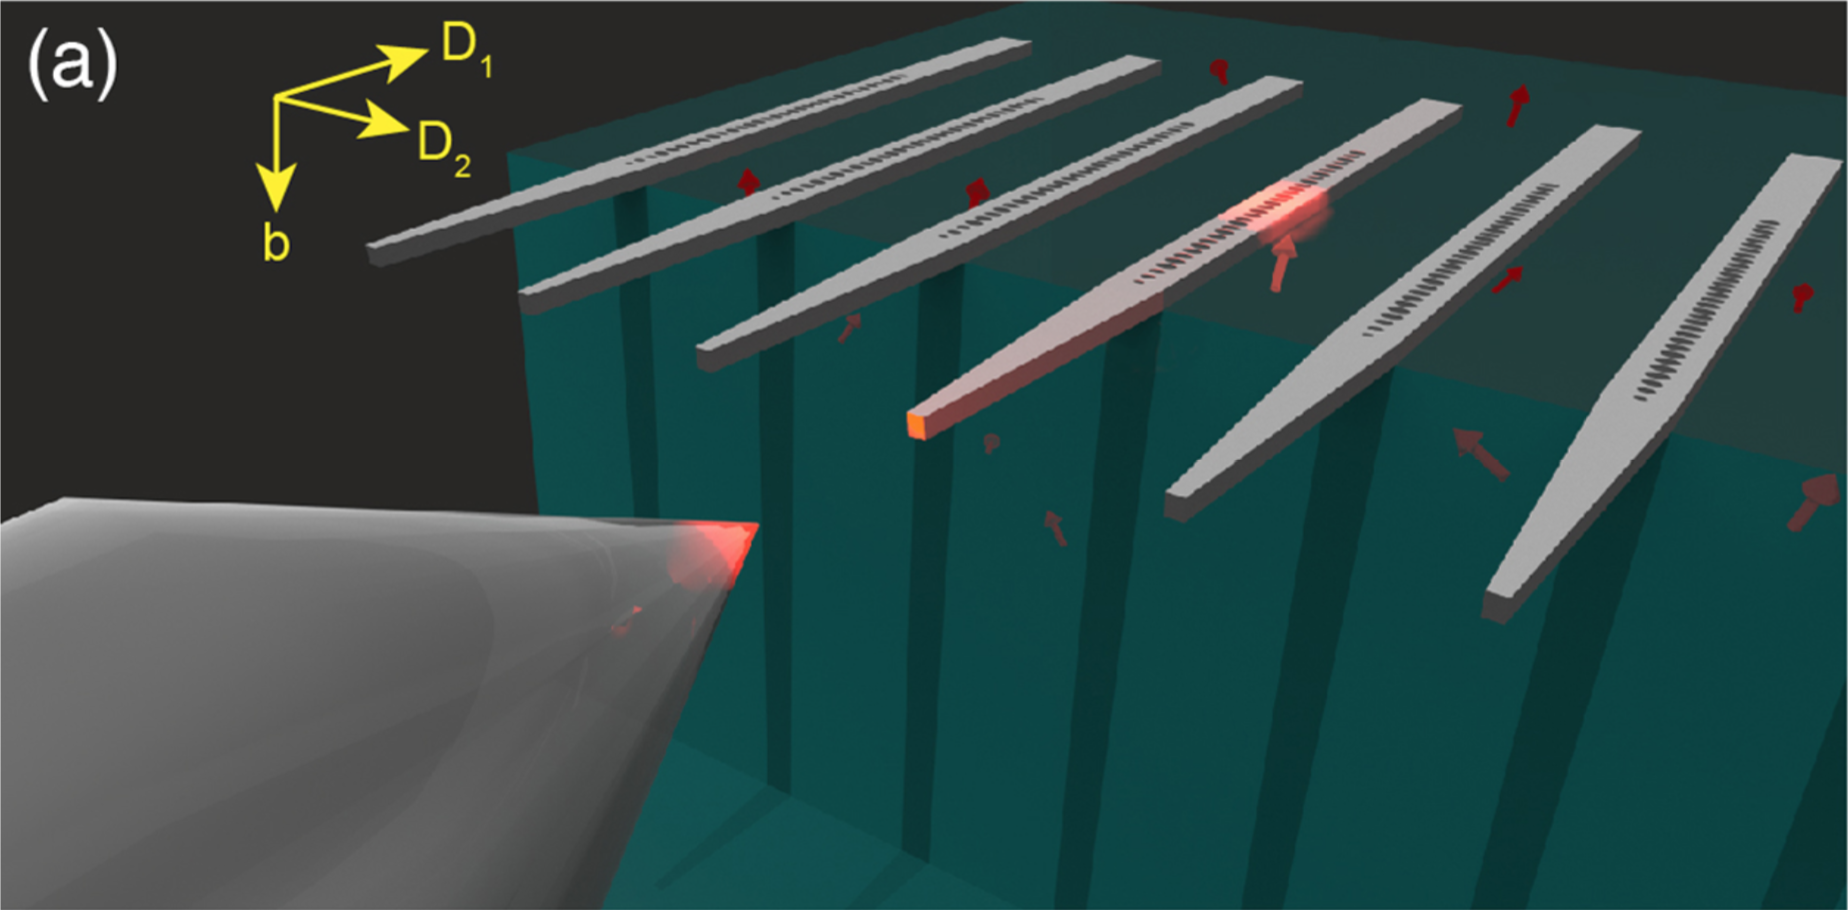
\includegraphics[width=0.8\textwidth]{Nanophotonics}
  \caption{A lensed fiber couples into a silicon photonic cavity stamped on top of an \erbium[]-doped \YSO crystal. Red arrows represent the spins of \erbium ions in the crystal substrate. Figure from \cite{Dibos2017}.}
  \label{fig:cavity}
\end{figure}


Previous work by the Thompson lab has shown that by stamping silicon nanophotonic cavities on top of crystals doped with \erbium ions, the emission rate can be enhanced by 600 times via the Purcell effect \cite{Dibos2017}. Figure \ref{fig:cavity} shows a graphic of this scheme. This approach is very promising - however, the crystal substrate could be improved in numerous ways. For one thing, this work used \YSO[], a crystal with relatively strong nuclear spins. These nuclear spins substantially limit the coherence times of the \erbium spin qubits embedded in the crystal. Another other issue is that the density of \erbium ions is high enough in the bulk-doped \YSO that tens to hundreds of ions couple to the cavity, preventing simple frequency-based resolution of the different ions each cavity couples to, and reducing coherence times further due to electric dipole interactions between nearby \erbium ions. Finally, a different crystal field configuration could potentially increase the emission rate further, by increasing the matrix element between the ground and excited state wavefunctions.\footnote{The \erbium telecom transition is electric dipole forbidden. Small perturbations to the electronic wavefunctions can thus make substantial relative differences to the matrix element between the ground and excited states. The spectroscopic properties of \erbium are discussed in more detail in Section \ref{sec:spectr-prop-erbi}.}

Unfortunately, using bulk doping methods it is impossible to grow crystals with lower concentrations of \erbium than in this previous work \cite{Dibos2017}. The Thompson lab has thus turned to ion implantation to achieve lower doses of \erbium in new potential crystal hosts.\footnote{Ion implantation is a process by which ions are accelerated into the surface of a crystal, and become lodged in the structure of the crystal. More information on this process is given in Section } Last fall, it was shown that \erbium could be successfully implanted in \TiO[]. The implanted \erbium had narrow optical linewidths, and \TiO has no nuclear spins, so this was an exciting result \cite{Phenicie2019}. However, the quality factor of photonic crystals on \TiO could never be made high enough, likely due to the poor telecom transparency of \TiO[].

In the interests of discovering better potential host crystals, a large batch of crystals was implanted with \erbium ions. For all these implanted crystals, it was necessary to determine experimentally whether \erbium was visible in the crystal, and if so, to determine its spectral properties to begin understanding how \erbium ions in this crystal would perform for single ion applications. Where are the emission and excitation lines? How bright and broad are they? What can we learn about how the \erbium ions are sitting in the crystal lattice? These are the questions that motivate this work. Before laying out our methods and results, we first provide some theoretical background about \erbium and crystals.

\section{Spectroscopic Properties of \erbium in Solid State Hosts}
\label{sec:spectr-prop-erbi}

Due to its telecom optical transition, \erbium has a long history of use as a dopant to make telecom wavelength fiber amplifiers.\footnote{Our spectroscopy experiment, in fact, uses an erbium-doped fiber amplifier (EDFA).} This optical transition is between the $^{4}I_{15/2}$ ground state, and an excited state $^{4}I_{13/2}$. This notation, known as spectroscopic notation, takes the form $^{2S+1}L_{J}$, where $S$ is the total spin momentum, $L$ is the total orbital momentum (specified as a letter, $S, P, D,$ etc., where $I$ corresponds to a total orbital momentum of 6), and $J$ is the total angular momentum. 

\begin{wrapfigure}{r}{0.5\textwidth}
  \centering
  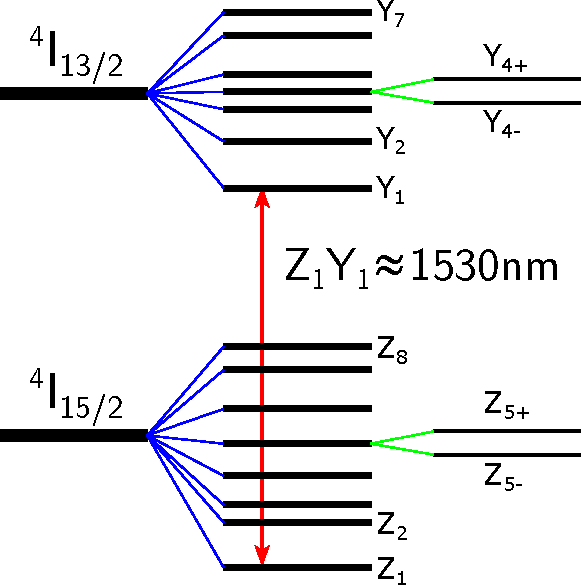
\includegraphics[width=0.48\textwidth]{EnergyLevelDiagram}
  \caption{Diagram showing the Stark splitting due to electric fields within the crystal (blue) and the Zeeman splitting in an applied magnetic field (green). The transition between the lowest ground and excited state levels, labelled in red, typically falls around 1530 nm.}
  \label{fig:energyleveldiagram}
\end{wrapfigure}

There are two consequences to this. One is that, because these $4f$ states lie closer to the nucleus than the $5d$ states which populate earlier, they are relatively shielded from phonons in the crystal. This makes \erbium and other rare-earth ions with this property desirable for building quantum memories, as the coherence times of the optical electrons are unusually good. The second consequence is that this transition is electric-dipole forbidden, as the total angular momentum $L$ is the same in the ground and excited states. This means that the transition is quite slow, with excited state lifetimes on the order of ten milliseconds (as previously discussed). For quantum network applications, this is less than desirable, and one of the principal motivations for the use of silicon photonic cavities. 

Both the ground state and the excited state are degenerate, 16- and 14-fold respectively. In solid state hosts, the crystal fields split these degeneracies via the Stark effect into $J+1/2$ Kramer's doublets. We label the ground state Stark-shifted doublet states with $Z_{1}$ to $Z_{8}$, and the excited state doublets with $Y_{1}$ to $Y_{7}$. In the presence of an applied magnetic field, these doublets themselves are split by the Zeeman effect, and the energy levels can become entirely nondegenerate. This splitting is shown in Figure \ref{fig:energyleveldiagram}. In this work, we ignore the Zeeman splitting, and focus on identifying how the electric field inside the crystal environment shifts the energy levels. 

Because the excited state lifetime of this system is so long, the natural linewidth is quite small. As a result, at low temperatures, the primary line broadening is inhomogeneous, a consequence of slight variations in the locations of different \erbium ions in the crystal, or slight deformations of the crystal field around them.


\section{Crystal fields}
\label{sec:crystal-fields}

The problem of modeling the effects of crystal fields on the spectra of ions is an old one, and tools exist for approaching it. First, we make use of the central field approximation, which roughly states that the repulsive potential an electron feels due to the other electrons is spherically symmetric. Thus the radial component of the wavefunctions decouples from the angular component, and focus can be turned to the angular component. The key idea underlying crystal field modelling is then decomposing the electric field of the crystal into a sum of spherical harmonics centered on the atom whose perturbations you are trying to measure. In other words, the crystal field hamiltonian is expressed as 
\begin{equation}\label{eq:3}
  H_{CF} = \sum_{k, q}B_{q}^{k}C_{q}^{(k)},
\end{equation}
where $B_{q}^{k}$ are parameters to describe how much of each spherical harmonic is present, and $\mathbf{C}^{(k)}$ are the tensor operators of spherical harmonics \cite{Liu2006}.

The next step is to pick a basis of quantum numbers for describing the angular component of the wavefunctions. The true good quantum numbers in general depend on the relative strength of the electrostatic forces in the atom versus the spin-orbit coupling. However, since the crystal field perturbation will take the form of spherical harmonics, it makes sense to use a basis of simple spherical harmonic wavefunctions. Thus, we use the basis $\ket{l\tau SLJM}$, where $l$ has to do with the radial part of the wavefunction $nl$, $S$ is the total spin momentum, $L$ is the total orbital momentum, $J$ is the total angular momentum $S+L$, and $M$ is the ``magnetic quantum number'' ranging from $-J,-J+1,...,J$, and $\tau$ is a seniority number to distinguish states with the same $S$ and $L$ which can't be otherwise distinguished \cite{Liu2006}.

Having decided on a basis, we do perturbation theory with the crystal field Hamiltonian. This involves computing the matrix elements, which are given by
\begin{equation}\label{eq:4}
  \bra{l\tau SLJM} H_{CF} \ket{l\tau' S'L'J'M'} = \sum_{k, q} B_{q}^{k}(-1)^{J-M}\Bigg(\begin{array}{c c c}J & k & J' \\ -M & q & M'\end{array}\Bigg)D_{J}^{k},
\end{equation}
where
\begin{align}
  D_{J}^{k} =
  & (-1)^{S+L'+J+k}[(2J+1)(2J'+1)]^{1/2}
    \Bigg\{\begin{array}{c c c} J & J' & k \\ L' & L & S \end{array}\Bigg\} \nonumber \\
  & \times \bra{l\tau S L } \mathbf{U}^{(k)}\ket{l\tau' S' L'}(-1)^{l}(2l + 1)
    \Bigg(\begin{array}{c c c} l & k & l \\ 0 & 0 & 0\end{array}\Bigg) \label{eq:5}                                                               
\end{align}
In the above equations, the $()$ and $\{\}$ quantities are 3- and 6-$j$ symbols, a notatation for representing Clebsh-Gordan coefficients. The $\mathbf{U}^{(k)}$ operator is the reduced matrix element of a unit tensor (see \cite{Wybourne1965} for more information). The key conclusion is that these matrix elements can be evaluated exactly and reduced to known linear combinations of the crystal field parameters $B_{q}^{k}$. Calculating the spectrum for a given set of crystal field is then only a matter of diagonalizing the matrix of the crystal field Hamiltonian. As a consequence, if the number of known energy levels is more than the number of unknown crystal field parameters, the crystal field parameters can be found conclusively.

In general, the number of crystal field parameters is infinite. However, various symmetries of the crystal can eliminate many of the possible parameters. For example, if the rare earth ion sees a crystal environment with cubic symmetry, only four crystal field parameters can be nonzero, $B_{4}^{0}$, $B_{4}^{4}$, $B_{6}^{0}$, and $B_{6}^{4}$, and only two of these are actually independent. Thus the problem is a two-parameter one. Lea, Leask and Wolf show an efficient way of calculating the crystal field matrix for diagonalization, 
\begin{equation}\label{eq:7}
  H = B_{4}(O_{4}^{0}+ 5\cdot O_{4}^{4}) + B_{6}(O_{6}^{0}-21\cdot O_{6}^{4}),
\end{equation}
where $O_{4}^{0}$, $O_{4}^{4}$, $O_{6}^{0}$ and $O_{6}^{4}$ are $2J+1$ dimensional constant matrices (for their exact form see \cite{Lea1962}). The upshot of this for our purposes is that the crystal field environment that \erbium ions experience in cubic crystals can potentially be determined exactly, enabling a complete description of the eigenstates of the \erbium optical electron. % In Section \ref{sec:mgo} we use this model to study \erbium in MgO, a crystal with cubic symmetry.


%%%%%%%%%%%%%%%%%%%%%%%%%%%%%%%%%%%%%%%%%%%%%%%%%%%%%%%%%%%%


\chapter{Methods}

\section{Sample preparation}
\label{sec:sample-preparation}

\subsection{Ion implantation}
\label{sec:ion-implantation}

There are many ways to dope ions into crystals. Previous work made use of so-called ``bulk-doping,'' a process where the crystal (in this case, \YSO[]) is grown with small amounts of \erbium in it. Unfortunately, for chemical reasons the minimum concentration of \erbium possible with bulk doping is still higher than is desirable for single-ion applications. Ion implantation is a method for doping in arbitrarily low quantities of an ion. Sing ions of the desired are separated into gas. These floating single ions are then accelerated into the target crystal with a powerful electric field. The number of ions that end up in the crystal can be measured via the current between the crystal and the ion source. 

\subsection{Annealing}
\label{sec:annealing}

Annealing is a process where crystals are heated to a temperature high enough that their structure can shift slightly, and then gradually cooled back down to room temperature. Annealing can be helpful in repairing structural damage like the damage done by ion implantation. In \cite{Phenicie2019}, the authors showed that annealing increased the implantation yield and reduced optical linewidths in \erbium implanted in \TiO[.] For all tested samples, annealing is a possible next step (provided the crystal can withstand it). If \erbium is visible, annealing might reduce linewidths, and if \erbium is not visible, annealing might increase the yield so that it is visible. 

\subsection{Polishing and photonic crystals}
\label{sec:polishing}

For our applications, it is important that the crystal hosts can be polished, as the photonic crystal cavities we use are attached to the top of the crystal purely through van der Waals forces. This method only works if the surface is sufficiently smooth. 

\section{Photoluminescence excitation spectroscopy}
\label{sec:phot-excit-spectr}

Photoluminescence excitation spectroscopy (PLE) is a spectroscopy technique wherein the sample is exposed to a tunable excitation laser, and the fluorescence from the sample is collected and measured. In principle, it measures the same physical properties as absorption spectroscopy. However, it is more effective for detecting extremely small doses of a material (as we are dealing with here) because rather than measuring a small signal against a large background, it measures a small signal against almost no background.

PLE spectroscopy measures how much light the sample can absorb and reemit at each wavelength in a scan. Physically, this corresponds to measuring the difference between the energies between the occupied ground states and the energies of the excited states. In theory, there will be excitation peaks at every energy $E_{nm}$ for which there is a transition 
\begin{equation}\label{eq:6}
E_{nm} = Y_{m}-Z_{n}.
\end{equation}
However, the relative strengths of these peaks are modulated by several factors. At different temperatures, the ground states will have different occpancies according to the Boltzmann distribution. The matrix elements between different $Z$ and $Y$ level states can be greater or lesser, which will influence the brightness of the observed transition. Finally, the linewidths of the transitions affect their brightnesses. When the natural linewidth is much smaller than the inhomogeneous linewidth due to environmental factors, only a small fraction of the ions are addressed by the laser at a given moment. On the other hand, as the natural linewidth increases, the excitation efficiency falls, and the line can also become weaker. The balance of these forces can be be unpredictable. Moreover, the laser power is not consistent across all wavelengths due to wavelength-dependent changes in the polarization. Thus, it is currently difficult to draw precise quantitative conclusions based on the relative heights of different excitation peaks. 

\begin{figure}[t]
  \centering
  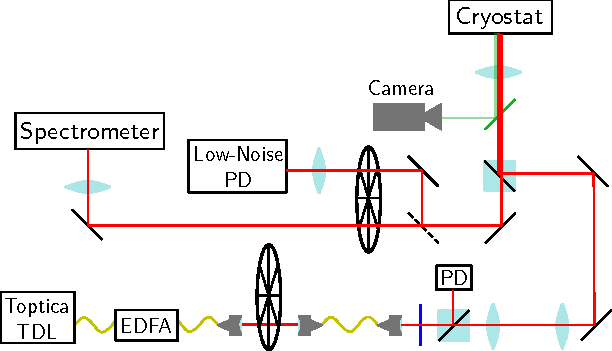
\includegraphics[width=0.9\textwidth]{PLESetupDiagram.pdf}
  \caption{Schematic of our spectroscopy experiment. A half-wave plate is marked in blue, and a dichroic mirror is marked in green. }
  \label{fig:ple}
\end{figure}

Our PLE setup is shown in Figure \ref{fig:ple}. A tunable diode laser is amplified by an erbium-doped fiber amplifier up to \notetoself{200 mW?}. The laser is then passed through a chopper. A half-wave plate (blue) at the output of the fiber enables coarse control over the polarization of the laser before it passes through a polarizing beamsplitter. A photodiode measures the light rejected by the PBS, informing the rotation of the HWP. The laser then passes through a beam expander consisting of two lenses, before reflecting off a PBS towards the vapor cryostat containing the sample. Before the cryostat the laser passes through a lens which focuses it onto the sample surface. A camera, which is added to the beam path with a dichroic (green), helps aim the laser at the sample.

The reflected excitation laser is mostly rejected from continuing down the measurement beampath by virtue of the PBS. Fluorescence from the sample, which has random polarization, makes it through this PBS with 50\% attenuation. The measurement beampath is then directed either to a low-noise photodiode, or to the array detector spectrometer, by inserting or removing a mirror (dotted line). Before measurement, the light passes through a second chopper set to be exactly out of phase with the first, so that residual excitation light is further rejected.\footnote{Since the excitated state lifetime of the \erbium ions is on the order of ms, fluorescent emission continues to be visible for several ms after the excitation laser is blocked.}

When the light is directed into the low-noise photodiode, we are performing pure PLE spectroscopy. There are two modes in which this can be operated. By directing the PD signal to a lock-in amplifier tuned to the frequency of the chopper, we can achieve an extremely low signal-to-noise ratio. This enables the measurement of the smallest signals we can observe with this setup. Alternatively, the PD output can be measured directly, enabling direct observation of the decay of the fluorescence, and thus the excited state lifetime.

In the next section, we discuss the array detector spectrometer and the measurements performed when the signal is instead directed into the other beam path.

\section{Emission spectroscopy with an array detector}
\label{sec:emiss-spectr-with}

Emission spectroscopy is a different form of fluorescence spectroscopy, where instead of scanning the wavelength of the excitation laser, you measure the frequency composition of the fluorescence itself. In our experiment, this is done by focusing the fluorescence into a thin slit, which spatially separates the different wavelengths of light, and then imaging this spatial spectrum onto an array of photodetectors. Thus the readout of each bin of the array detector corresponds to the emission at a different wavelength of light.

The emission spectrum is different from the excitation spectrum, due primarily to the fact that higher energy states have lower occupation at lower temperatures. In principle, all of the same transitions are visible; however, while the $Z_{1}Y_{1}$ and $Z_{1}Y_{2}$ transitions might appear equally bright while performing excitation spectroscopy, the former might be substanitally brighter when performing emission spectroscopy if the thermal occupation of $Y_{1}$ is substantially higher than $Y_{2}$. Thus, the emission and excitation spectra might look very different, especially at low temperatures.

This is why it can be advantageous to measure both at the same time. By measuring the emission spectrum for a range of different excitation wavelengths, a so-called ``2D spectrum'' can be obtained. Especially in situations where \erbium is sitting at multiple different sites in the crystal and thus multiple spectra are accessible, this additional dimension of resolution can be helpful in distinguishing the different spectra.

Before measuring 2D spectra, an excitation scan is performed to identify the excitation wavelengths at which emission is visible. Then 2D scans are performed on the regions where features were visible. 

\section{Peak finding and assignment}
\label{sec:peak-find-assignm}

The processing of 2D spectra consists of several steps. First, a moving window smoothing is performed on the two dimensions, one after another, iteratively. The number of iterations and the size of the windows are adjusted to reduce the number of non-physical local maxima in the data, but are kept as low as possible to avoid decreasing the resolution of the data. Typical values are two iterations with windows that are three bins wide.

\begin{figure}[b]
  \centering
  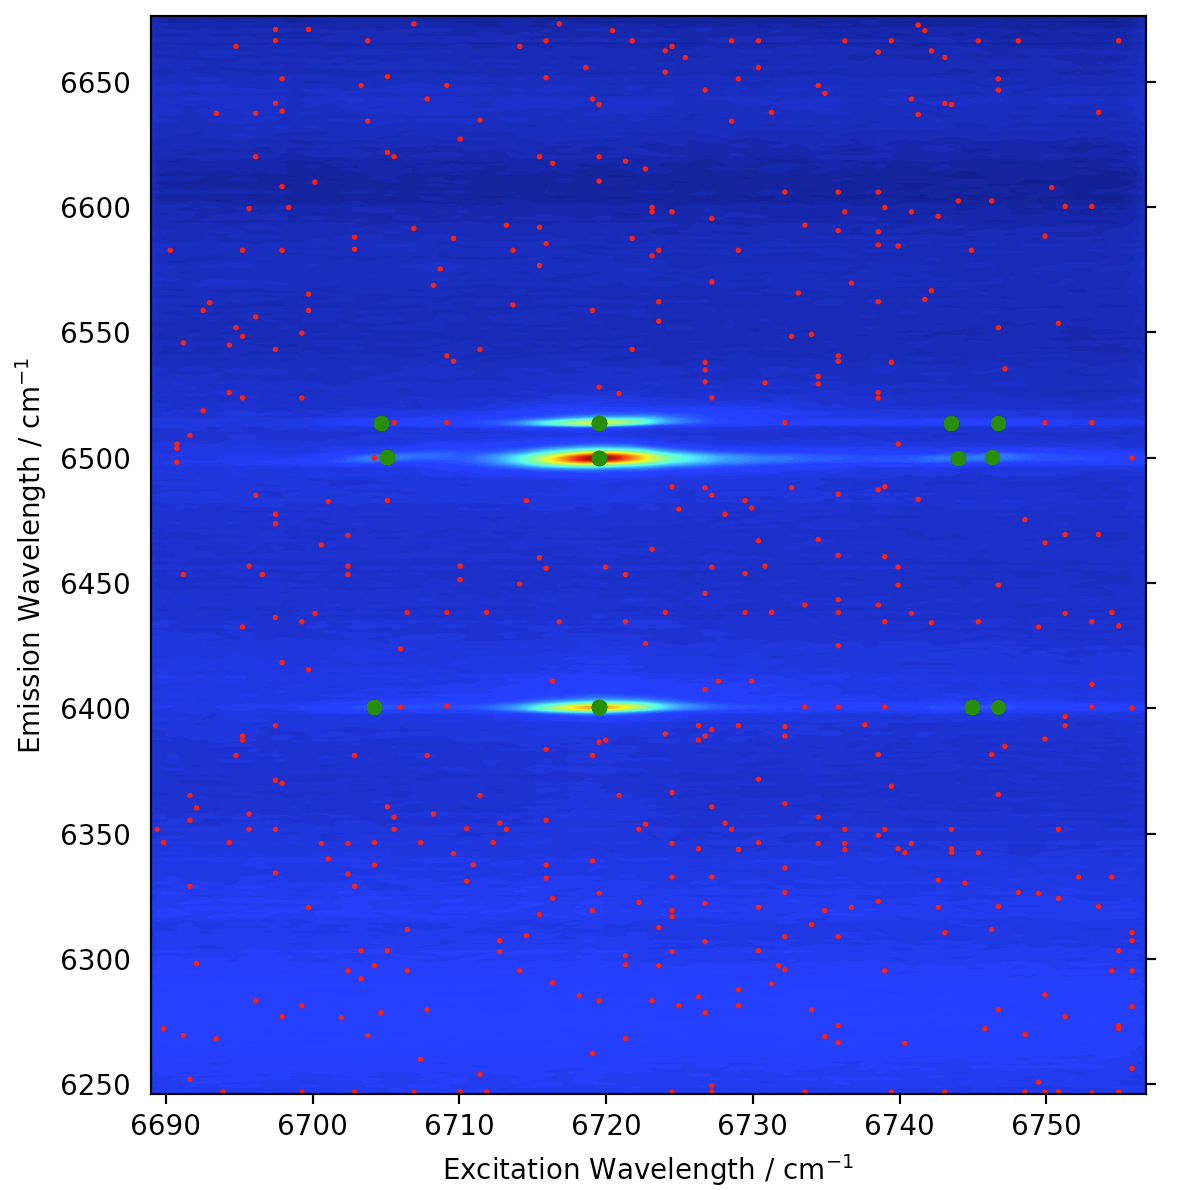
\includegraphics[width=0.47\textwidth]{PeakFinding}
  \hfill
  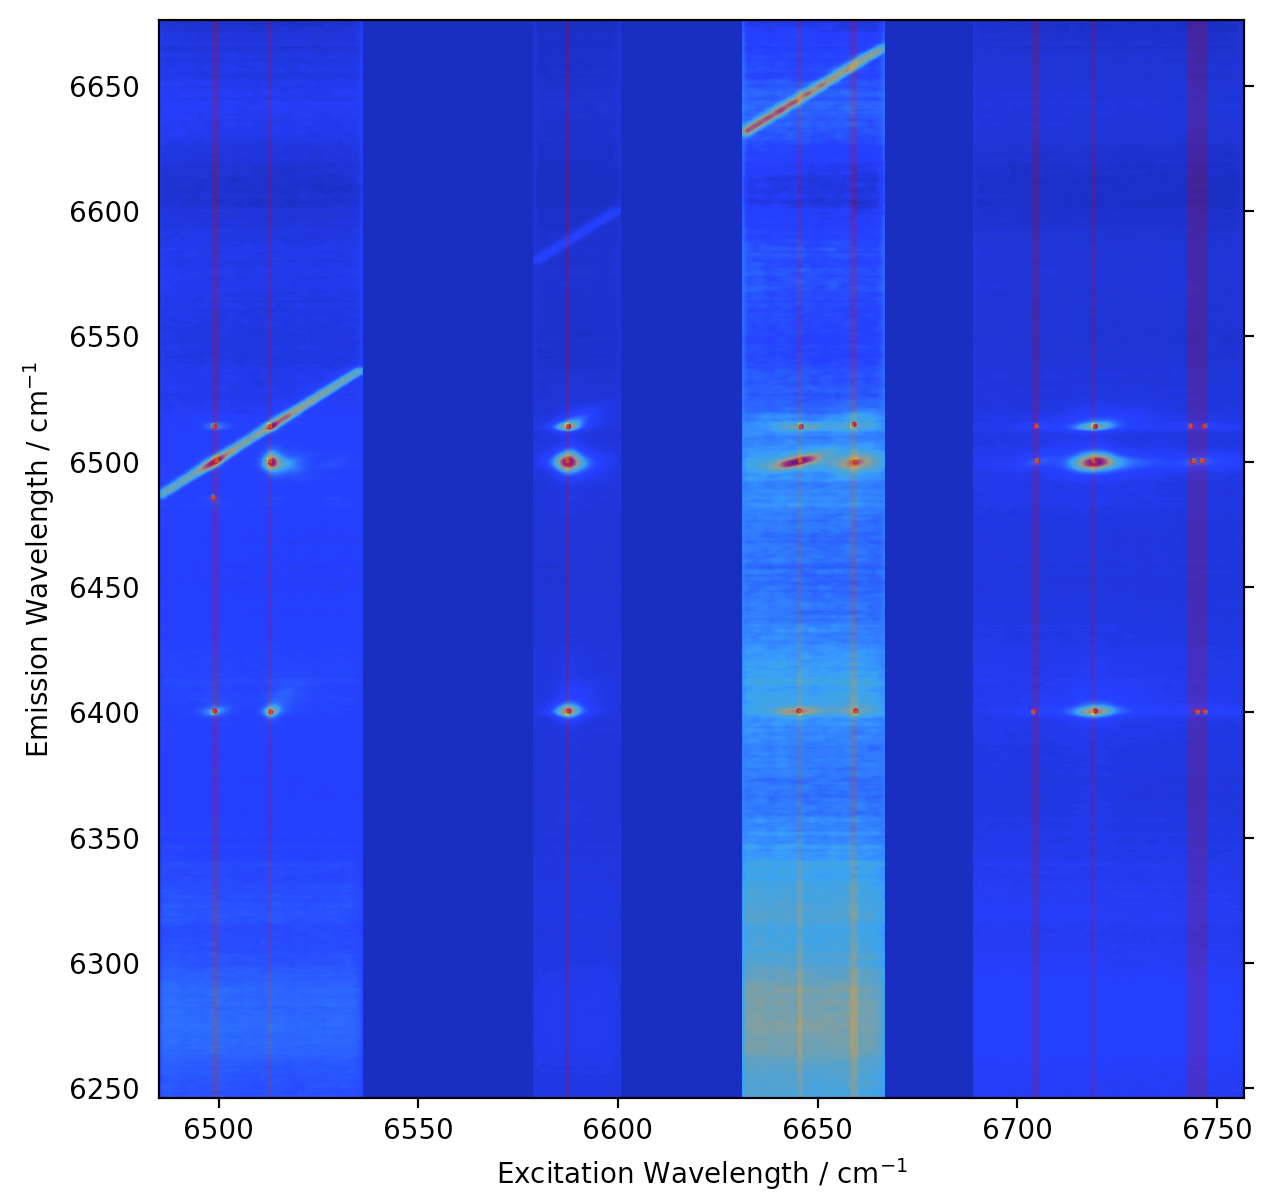
\includegraphics[width=0.47\textwidth]{LineSorting}
  \caption{Left: a screenshot of peak sorting. Red dots are all potential peaks, green dots are the ones that have been manually selected as belonging to physical features. Right: a screenshot of grouping excitation lines into different sites. In the given figure, all lines belong to the same site.}
  \label{fig:manual}
\end{figure}

Next, all the local maxima in the 2D spectrum are identified. The maxima are then sorted by hand, keeping only those which correspond to physical peaks. A screenshot of this process is provided in Figure \ref{fig:manual}. In the future, it would be preferable to do this filtration automatically, but it turns out to be a fairly difficult task to reject all the false peaks and accept all the real peaks, as the real peaks are often barely larger than the background noise.

Once the real peaks are identified, they are sorted into different sites. This is also done manually, as depicted in Figure \ref{fig:manual}, by clicking on the vertical bins which contain peaks belonging to a given site to identify excitation lines. The emission lines are subsequently identified in the same way. From the emission and excitation lines, the energy level structures of the ground and excited states can be inferred.



%%%%%%%%%%%%%%%%%%%%%%%%%%%%%%%%%%%%%%%%%%%%%%%%%%%%%%%%%%%%

\chapter{Characterization of new hosts}


\section{MgO}
\label{sec:mgo}

\begin{figure}[t]
  \centering
  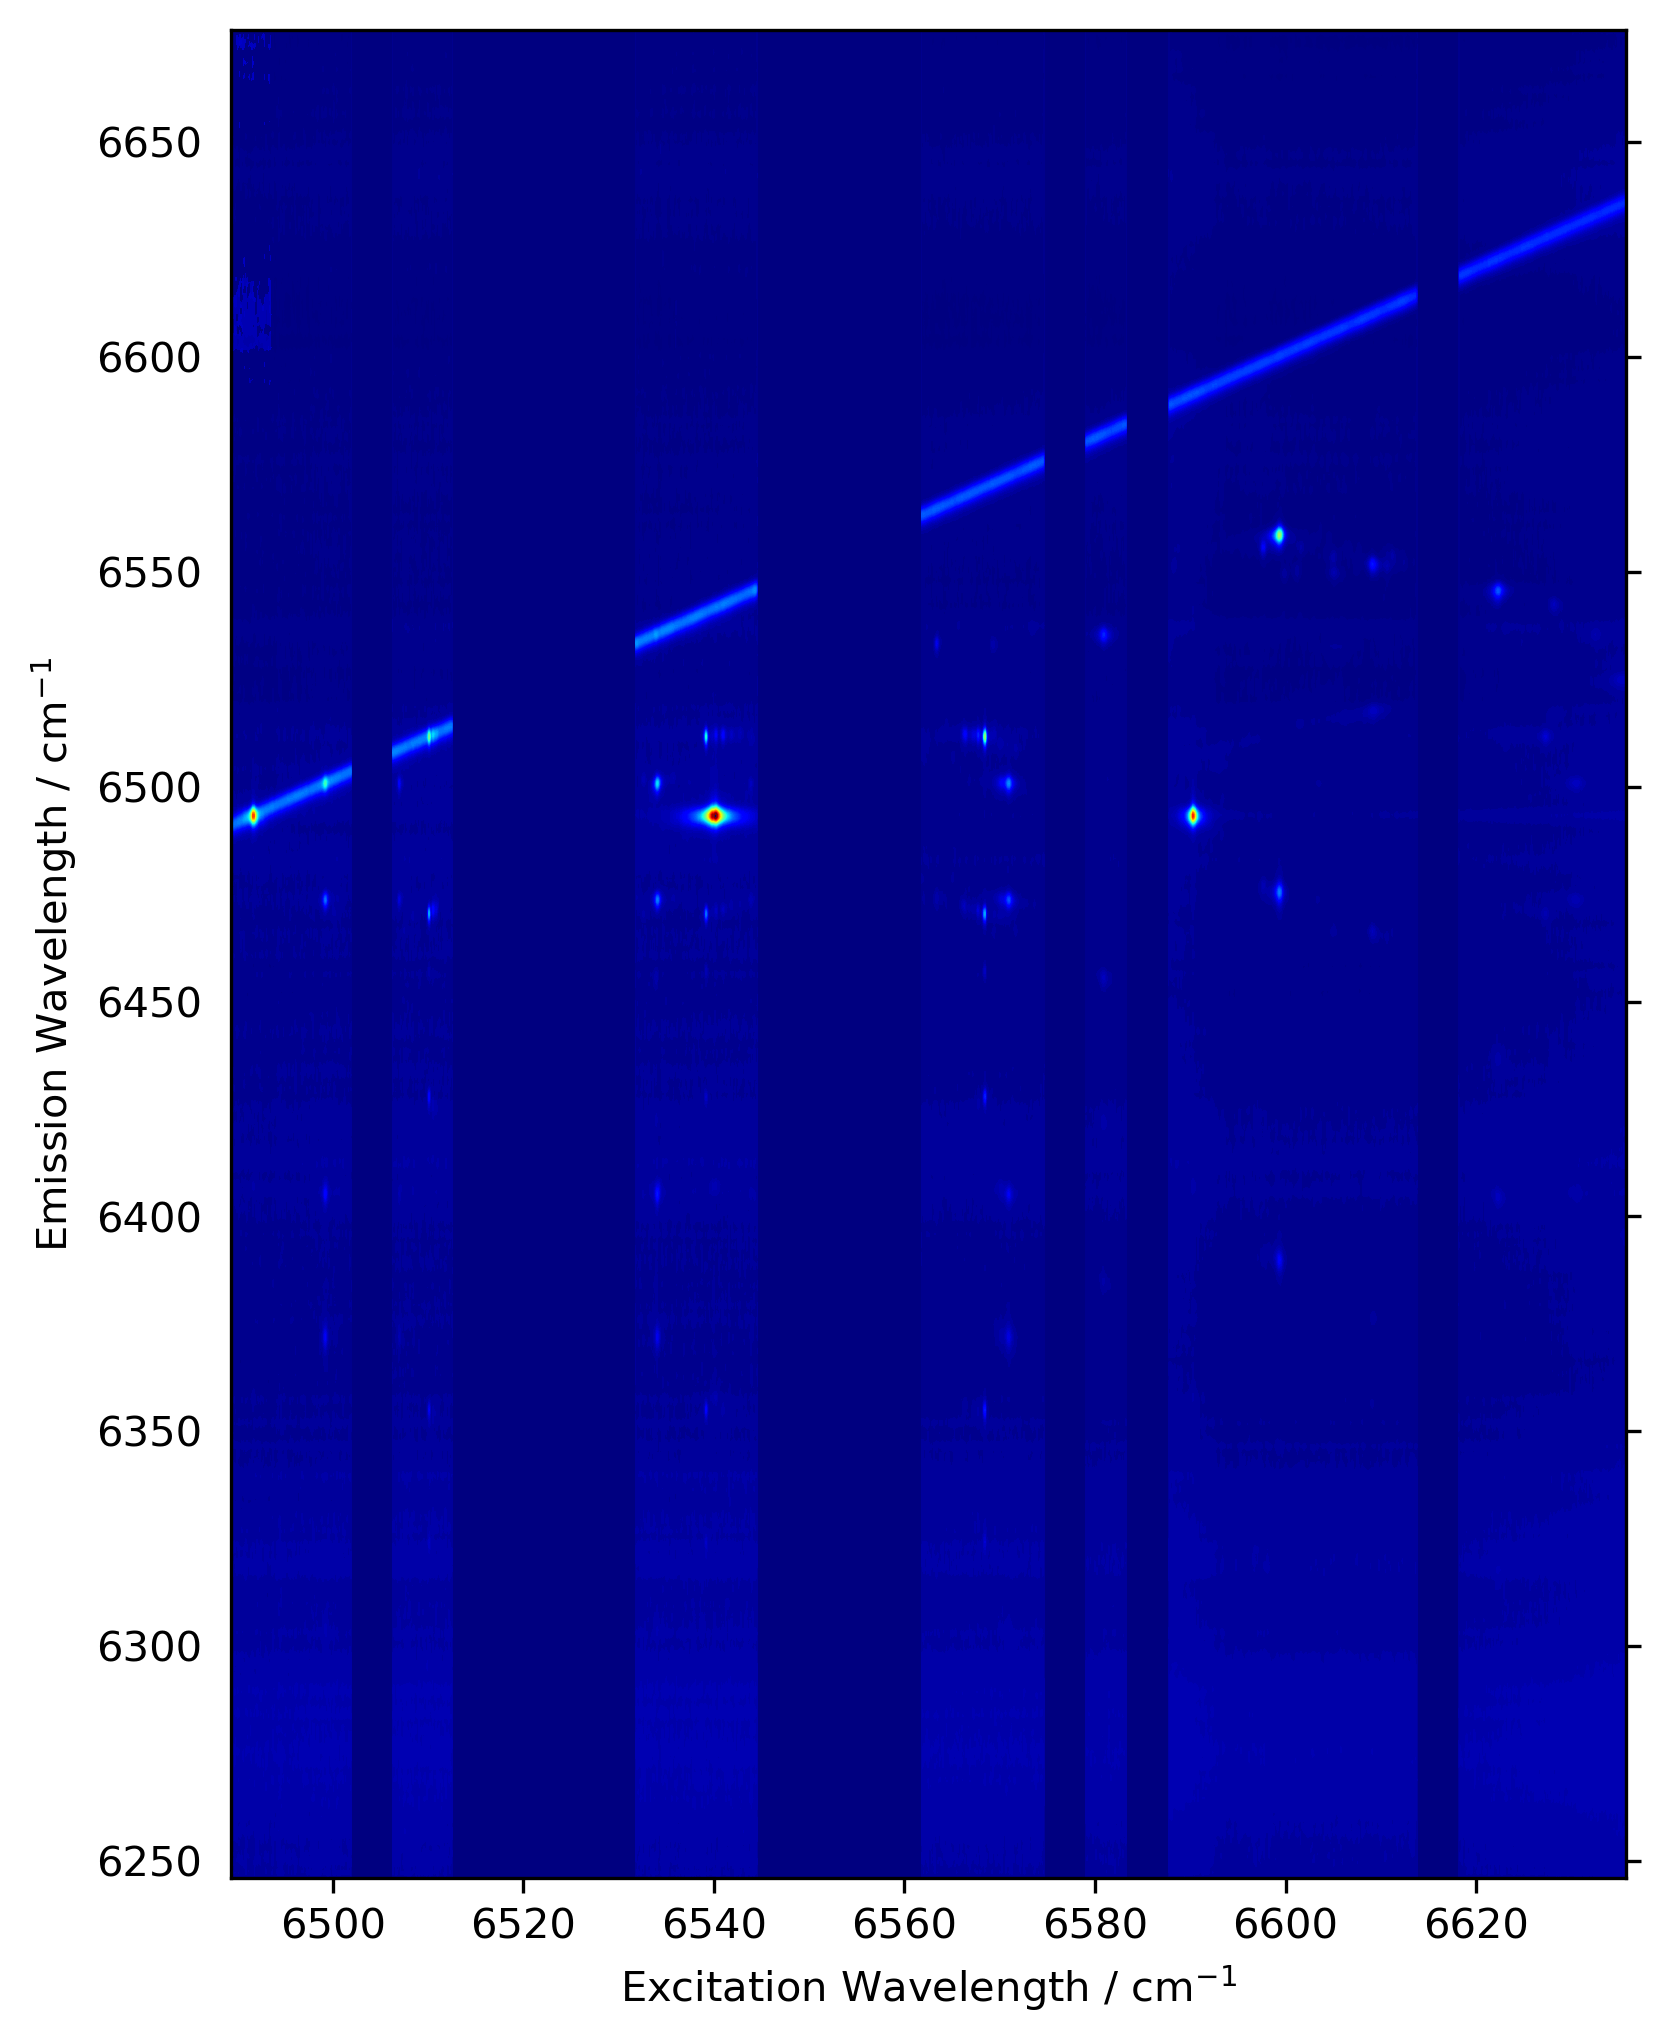
\includegraphics[scale=1]{JinD_spectrum_13K}
  \caption{Excitation-emission spectrum of MgO at 13K.}
  \label{fig:mgospectrum}
\end{figure}

\subsection{Sample preparation}
Implanted with $10^{19}$ dose \notetoself{find out units on this}. Unannealed.

\subsection{Structure}
Magnesium oxide (MgO) is a cubic lattice consisting of O$^{2-}$ ions and Mg$^{2+}$ ions held together by ionic bonding. There are three sites with cubic symmetry: the two substitutional sites have cubic symmetry, as does the interstitial site in the center of the cube. Because the crystal must remain net neutral, there might be some restructuring of the surrounding environment to compensate the introduction of the additional positive charge from the implanted \erbium ion. This may disturb the symmetries of the crystal.

\newpage 
\subsection{Energy levels}
The spectrum for MgO is fairly complicated, with at least four clearly different sites contributing to the excitation-emission spectrum. The experimentally determined energy levels for each of these sites is listed in Table \ref{tab:mgolevels}, and plotted over the spectra in Figures \ref{fig:mgosite1}, \ref{fig:mgosite2}, \ref{fig:mgosite3}, and \ref{fig:mgosite4}. These figures show excitation and emission from new $Z$ and $Y$ levels beginning to appear at higher temperatures.

Our energy level assignments are also supported by the temperature-dependent data in Figure \ref{fig:mgotemp}. These figures show the emission spectra when exciting the $Z_{1}Y_{1}$ transition of the different sites, normalized so that emission at $Y_{1}Z_{1}$ is equal to 1. The other features identified as emission from $Y_{1}$ remain the same height relative to $Y_{1}Z_{1}$. The features identified as emission from higher $Y$ levels, on the other hand, get brighter as the temperature increases, demonstrating that their thermal occupation has increased. An important assumption in this situation is that emission is slow enough that the excited state electrons thermalize fully before decaying. This assumption is supported by the fact that the relative heights of the peaks in the emission spectrum are independent of the excitation transition at which they are observed.

\begin{wrapfigure}{r}{0.5\textwidth}
  \centering
  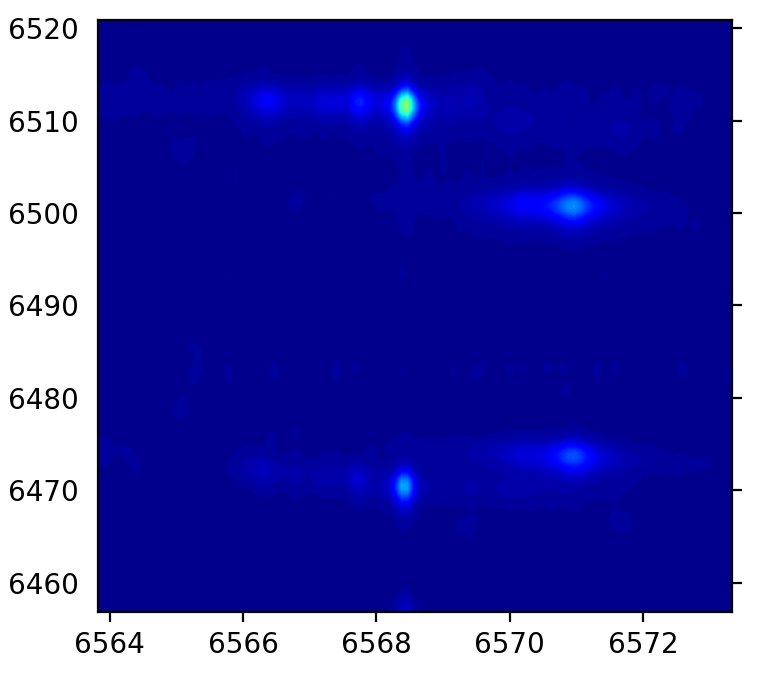
\includegraphics[width=0.48\textwidth]{Site2Multiplicity}
  \caption{Detail plot of Site 2 side bands in the MgO excitation-emission spectrum at 13K.}
  \label{fig:site2sidebands}
\end{wrapfigure}

A few idiosyncracies are important to note for some of these sites. The $Z_{5}$ energy at Site 1 was never directly observed in the form of $Y_{1}Z_{5}$ emission like all the other $Z$ levels, and is hence listed in parenthesis. However, its location can be inferred from an emission line $Y_{3}Z_{5}$ which appears at higher temperatures. This peak can be seen emerging in Figure \ref{fig:mgosite1} and Figure \ref{fig:mgotemp}.

\begin{table}[t]
  \centering
  \begin{tabular}{| c | c | c | c | c |}
    \hline
    MgO & \multicolumn{2}{c|}{Site 1}& \multicolumn{2}{c|}{Site 2} \\
    \hline
    $n$ & $Z_{n}$ & $Y_{n}$ ($+6499$ \wn) & $Z_{n}$ & $Y_{n}$ ($+6510$ \wn) \\
    \hline 
    1 & 0.0 & 0.0 & 0.0 & 0.0 \\
    2 & 26.7 & 7.8 & 41.2 & 29.1 \\
    3 & 95.3 & 34.9 & 83.8 & 58.3 \\
    4 & 128.6 & 71.7 & 156.4 & 117.2 \\
    5 & (195.2) & 131.3 & 187.2 & * \\
    6-8 & * & * & * & * \\
    \hline \hline
    MgO & \multicolumn{2}{c|}{Site 3}& \multicolumn{2}{c|}{Site 4} \\
    \hline
    $n$ & $Z_{n}$ & $Y_{n}$ ($+6492$ \wn) & $Z_{n}$ & $Y_{n}$ ($+6557$ \wn)\\
    \hline 
    1 & 0.0 & 0.0 & 0.0 & 0.0  \\
    2 & * & (48.1) & 82.8 & 42.0 \\
    3 & * & (48.4) & 168.6 & *  \\
    4 & * & (98.6) & * & * \\
    5-8 & * & * & * & * \\
    \hline
  \end{tabular}
  \caption{Experimentally determined energy levels of MgO for all visible sites. Transitions not observed are marked with an asterisk. The level $Z_{5}$ in Site 1 is not directly observed, and thus marked with parentheses. The numbering of the $Z$ levels for Site 3 is somewhat uncertain (see the discussion in Section \ref{sec:linewidths-shapes}).}
  \label{tab:mgolevels}
\end{table}

Another idiosyncracy is that Site 2 exhibits numerous side bands in both excitation and emission at low temperatures. These extra peaks can be seen in Figure \ref{fig:mgosite2}, and a detail plot of some of them is given in Figure \ref{fig:site2sidebands}. The multiplicity of these peaks is too high for all of them to be associated with the same site. Thus, we conclude that they represent perturbations to the main Site 2, caused by small differences in the crystal structure some distance away from the \erbium ions. One possibility is that nearby Mg$^{2+}$ ions have been removed to compensate for the additional charge introduced by the \erbium ions, and that the different levels are due to different locations of these nearby Mg-vacancies in the crystal.

A third idiosyncracy has to do with the brightest peak in the entire spectrum, which belongs to Site 3, and falls at roughly 6540 \wn\ in excitation. This peak is bimodal, as shown in Figure \ref{fig:site3peaks}. There are two explanations for this distribution. Either these two peaks correspond to different levels in the same site, or they correspond to the same level at two sites which are very similar. To emphasize the uncertainty of the numbering of these peaks, they have been marked with parentheses in Table \ref{tab:mgolevels}.

\subsection{Crystal field modelling}
Unimplanted MgO has a cubic crystal structure. In an environment with cubic symmetry, there are only two free crystal field parameters, and thus the task of fitting an experimentally determined spectrum to theory is feasible (see Section \ref{sec:crystal-fields}). Interestingly, however, neither Site 1, Site 2, or Site 4 have energy levels consistent with a cubic crystal environment. From this, we conclude that charge compensation when \erbium replaces Mg$^{2+}$ necessitates changes to the crystal structure surrounding the \erbium which break the cubic symmetry of the environment. A likely candidate is the removal of nearby Mg$^{2+}$ ions, which can occur in line with the \erbium ion two sites away, or diagonally from the \erbium ion, or possibly farther away.

\begin{wraptable}{r}{0.5\textwidth}
  \centering
  \begin{tabular}{| c | c | c |}
    \hline
    $B_{4}$ & $B_{6}$ & SSE (cm$^{-2}$) \\
    \hline
    $-1.67\times 10^{-4}$ & $4.87\times 10^{-5}$ & $8.1\times 10^{-2}$ \\
    $1.51\times 10^{-2}$ & $-1.58\times 10^{-6}$ & $7.8\times 10^{-2}$\\
    \hline
  \end{tabular}
  \caption{Cubic crystal field parameters that reproduce the spectrum of Site 3 to within the resolution of the experiment.}
  \label{tab:crystalfieldparams}
\end{wraptable}

The spectrum of Site 3, on the other hand, can be reproduced by a cubic crystal field model. Table \ref{tab:crystalfieldparams} shows the two sets of crystal field parameters which give accurate\footnote{Where accurate is defined to mean that the sum of squared errors of the energy levels is within the tolerances of the spectrometer resolution, roughly 1 \wn.} reproductions of the energy levels observed in Site 3. The fitting of these parameters must be taken with a grain of salt; since Site 3 only has two nontrivial energy levels,\footnote{$Z_{2}$ and $Z_{3}$ are not different enough to count separately for our purposes.} it is not surprising that it was possible to fit two parameters effectively; the problem is not overdetermined. Further investigation is warranted. For example, given a set of crystal field parameters, it is possible to calculate the matrix element between the different states, and thus the theoretical brightness of each transition. If the theoretical transition strengths match the observed transition strengths, it would be stronger evidence for the accuracy of one of these sets of parameters.

Another route to inferring the remaining ground states of Site 3 is through the remaining visible emission lines in Figure \ref{fig:mgosite3}. As the temperature dependent data in Figure \ref{fig:mgotemp} show, these lower energy lines do not correspond to emission from $Y_{1}$, as they get relatively brighter with increasing temperature. By quantitatively studying the temperature dependence of their increasing brightness, we could deduce the $Y$ level from which they originate. From there, some of the remaining $Z$ levels could be calculated.


\subsection{Linewidths and shapes}
\label{sec:linewidths-shapes}
PLE scans of MgO were taken at 13, 32, 60, and 106K. Taking the level assignments discussed above, the excitation peaks corresponding to excitation from $Z_{1}$ to $Y_{n}$ for all visible $Y_{n}$ were located for all four sites. For each of these peaks, two profiles were fitted, a Gaussian profile and a Lorentzian profile. When the dominant source of broadening in a spectral line is homogeneous, its profile will be Lorentzian; when the dominant broadening is inhomogeneous, the profile will in general be Gaussian. Table \ref{tab:mgolinewidths} shows the results of these fits.

\begin{table}[t]
  \centering
  \begin{tabular}{|c| c| c | c | c | c | c | c | c|}
    \hline
    MgO & \multicolumn{4}{c|}{Site 1} & \multicolumn{4}{c|}{Site 2} \\
    \hline
    $n$ & 13K & 32K & 60K & 106K & 13K & 32K & 60K & 106K \\
    \hline
    1 & $0.27$ & $0.27$ & $0.42$ & $1.01$   & $0.06$   & $0.07$   & $0.15$   & $(0.29)$ \\
    2 & $0.13$ & $0.19$ & $0.33$ & $1.62$   & $(0.10)$ & $(0.11)$ & $(0.14)$ & *      \\
    3 & $0.33$ & $0.35$ & $0.57$ & $(1.03)$ & $0.12$   & $(0.14)$ & $0.17$   & $0.32$ \\
    4 & $0.47$ & $0.52$ & $0.81$ & *        & *        & *        & *        & *      \\
    5-8 & * & * & * & * & * & * & * & * \\
    \hline \hline
    MgO & \multicolumn{4}{c|}{Site 3} & \multicolumn{4}{c|}{Site 4} \\
    \hline
    $n$ & 13K & 32K & 60K & 106K & 13K & 32K & 60K & 106K \\
    \hline
    1 & $[0.23]$ & $[0.26]$ & $0.29$ & $0.41$ & $0.24$ & $0.26$ & $0.53$ & $1.17$ \\
    2 & $[0.84]$ & $[0.87]$ & $[0.91]$ & $1.04$ & $0.40$ & $0.46$ & $0.73$ & *      \\
    3 & $[0.82]$ & $[0.86]$ & $[0.89]$ & $1.01$ & *      & *      & *      & *      \\
    4 & $0.29$ & $0.30$ & $0.33$ & $0.57$ & *      & *      & *      & *      \\
    5-8 & * & * & * & * & * & * & * & * \\
    \hline
  \end{tabular}
  \caption{Fitted linewidths in \wn\ for all $Z_{1}Y_{n}$ excitation transitions in Sites 1, 2, 3, and 4, at 13, 32, 60, and 106 K. Peaks where a Gaussian distribution fit better than a Lorentzian based on the $R^{2}$ value of the fit are listed in parentheses. Peaks with bimodal lineshapes that required further analysis are marked with square brackets. Peaks that were not visible are marked with an asterisk.}
  \label{tab:mgolinewidths}
\end{table}

In general, the data were matched extremely well by one of these two distributions. Mostly, the best fits were Lorentzian, which is significant as it indicates that the inhomogeneous linewidths of these sites are quite small. For Sites 1, 3, and 4, the inhomogeneous linewidths must be less than 0.3 \wn\ FWHM at 13K, and for Site 2 they can be as low as 0.06 \wn. This is significant, as narrow inhomogeneous linewidths are desirable for our single-ion applications \cite{Dibos2017}.

\begin{figure}[b]
  \centering
  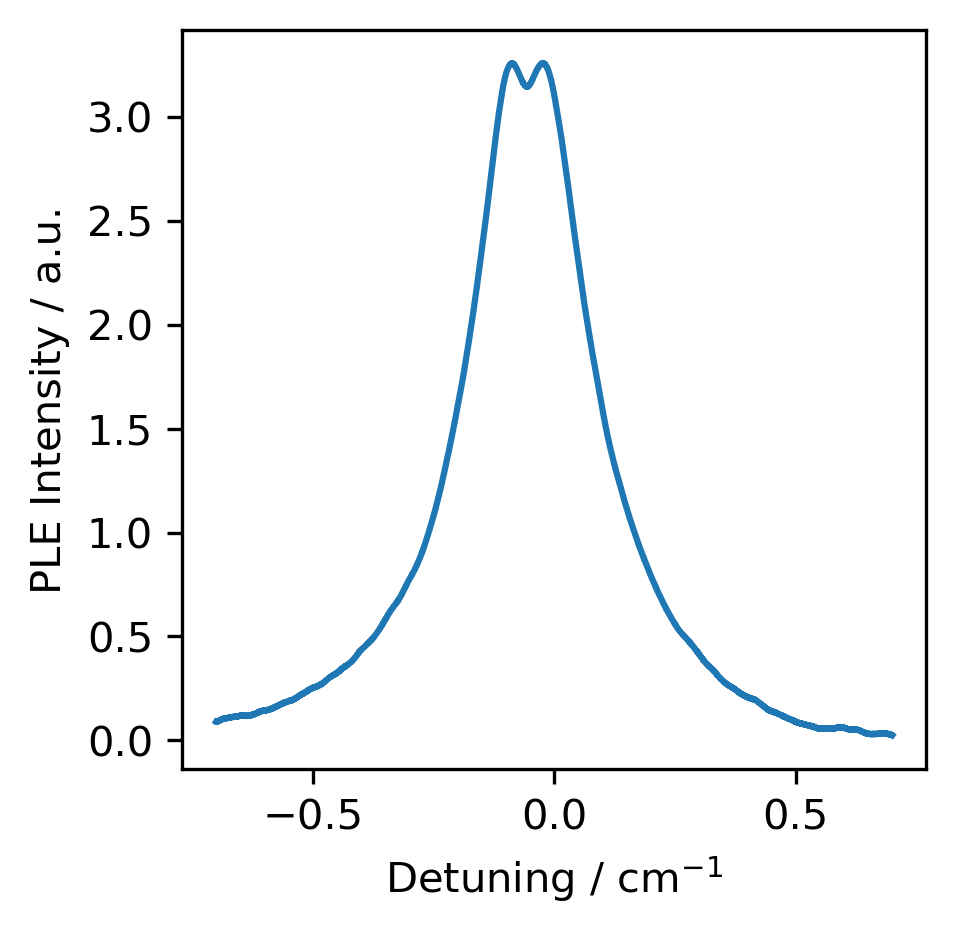
\includegraphics[width=0.48\textwidth]{Site3_y1}
  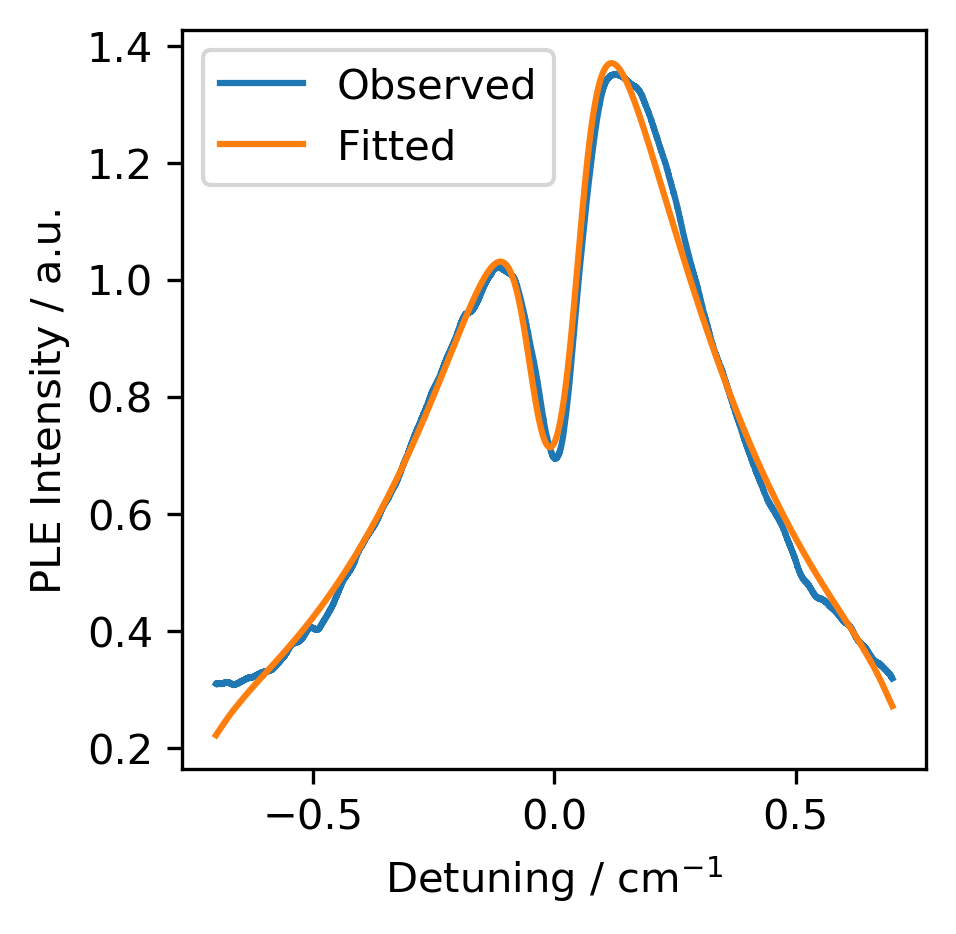
\includegraphics[width=0.48\textwidth]{Site3_y2}
  \caption{Excitation peaks at $Z_1Y_1$ (left) and $Z_1Y_2$ (right) in Site 3. The intensity profile discussed in Equation \eqref{eq:1} is fitted to the $Z_{1}Y_{2}$ data. Fitted model parameters are: $a_{1} = 2.3$, $\Delta_{1} = 0.05$, $\Gamma_{1} = 0.28$, $a_{2} = 1.6$, $\Delta_{2} = -0.05$, $\Gamma_{2} = 0.28$, $\Gamma_{3} = 0.0025$, $b = 0.12$}
  \label{fig:site3peaks}
\end{figure}

Two transitions ($Z_{1}Y_{1}$ and $Z_{1}Y_{2}$ in Site 3) had distributions that clearly did not match either Lorentzian or Gaussian distributions at all. These features are shown in Figure \ref{fig:site3peaks}. The distributions are clearly bimodal. In the case of $Z_{1}Y_{1}$, it would be possible to interpret the feature as two closely-spaced Lorentzian distributions. In the case of $Z_{1}Y_{2}$, however, the two halves of the distribution are clearly skewed away from the center. We believe this is due to a strong second-order Stark shift on these energy levels. 

To understand this, we first take a step back to discuss first-order Stark shifts and inhomogeneous broadening. The standard assumption underlying the Gaussian functional form associated with inhomogeneous broadening is that ions throughout the crystal experience different random electric fields $\mathbf{F}$, which are Gaussian distributed with zero mean. The energy levels are then shifted according to first-order perturbation theory, by diagonalizing the matrix $V$ given by
\begin{equation}\label{eq:2}
  (V)_{ij} = -\mathbf{F}e\bra{\psi_{i}}\mathbf{r}\ket{\psi_{j}},
\end{equation}
where the indices $i$ and $j$ run over all eigenstates with the same energy. The key takeaway of this is that the shifts are linear in the applied field $\mathbf{F}$. Thus, since the distribution of electric fields $F$ is Gaussian, so must be the distribution of energy level shifts.

However, if the electric dipole terms $\bra{\psi_{i}}\mathbf{r}\ket{\psi_{j}}$ of the eigenstates in question are all zero, there will be no first order Stark shift. In this case, we must go to second order in perturbation theory. The second-order shift to the energy of a state $E_{i}$ is 
\begin{equation}\label{eq:8}
E_{i}^{(2)} = \sum_{j\neq i }\frac{\bra{\psi_{i}}e\mathbf{F}\cdot\mathbf{r}\ket{\psi_{j}}\bra{\psi_{j}}e\mathbf{F}\cdot\mathbf{r}\ket{\psi_{i}}}{E_{i}^{(0)}-E_{j}^{(0)}}.
\end{equation}
Now, the perturbation is proportional to the square of applied electric field. Thus, still assuming a Gaussian distribution of fields, the distribution of perturbations is exponential. Whether the distribution lies to the left or right of zero depends on the sign of the second-order Stark shift.

Understanding this, the distribution on the right side of Figure \ref{fig:site3peaks} looks a lot like two exponentials with tails facing in opposite directions. We designed an dummy intensity profile $I$ which corresponds to two exponential distributions facing in opposite directions, convolved with a Lorentzian distribution to model the contribution of the natural linewidth. $I$ as a function of the detuning $x$ is given by \begin{equation}\label{eq:1}
  I(x) = b+N\int_{x'}dx'\frac{1}{x'^{2}+(\Gamma_{3}/2)^{2}}\Big(
    a_{1} D(x - \Delta_{1}) e^{-x/\Gamma_{1}} + a_{2}D(\Delta_{2}-x)e^{x/\Gamma_{2}}
  \Big) ,
\end{equation}
where $D$ is the Heaviside step function, $N$ is a normalization prefactor, $b$ is the background intensity, $\Gamma_{1}$-$\Gamma_{3}$ are linewidth parameters, and $\Delta_{1}$-$\Delta_{2}$ are the offsets of the two exponential distributions.

Figure \ref{fig:site3peaks} shows that the agreement between this fitted model and the data is very good. We thus conclude that this feature corresponds to two different features with opposite sign second-order Stark shifts. Whether these features belong to the same site or two different sites is unclear, but the former seems more likely than the latter due to their incredibly close spacing. The same question applies to the bimodal $Z_{1}Y_{1}$ feature at Site 3. For the purposes of simplicity, the $Z_{1}Y_{1}$ features has been treated as a single line throughout this analysis. However, due to their significant separation ($\sim 0.1$ \wn), the $Z_{1}Y_{2}$ features have been treated as two separate features, referred to as $Z_{1}Y_{2}$ and $Z_{1}Y_{3}$ throughout. To emphasize the uncertainty of this choice, the energy levels reported in Table \ref{tab:mgolevels} are marked with parentheses to indicate that the numbering is uncertain.

\subsection{Potential for single-ion applications}
The observation of \erbium ions implanted in MgO is very exciting, because MgO has several desirable qualities as a potential host crystal. Magnesium and oxygen both have stable isotopes with nuclear spin 0, so MgO can be made free of the nuclear spin problem that reduced coherence times in YSO. \erbium in MgO might therefore have substantially longer coherence times.

Another quality of MgO that made it an exciting candidate host was its high level of symmetry. A highly symmetric crystal will typically reduce the static electric dipole moment of an implanted ion, and thus its susceptibility to inhomogeneous broadening via the first-order Stark effect. Our results do indeed show very narrow inhomogeneous linewidths for several of the sites, especially Site 2, where the smallest observed linewidth was around $2$ GHz and appeared to be naturally broadened, indicating that the inhomogeneous linewidth is even lower. Interestingly, the only site that was inhomogeneously broadened at 13K was Site 3, the site which we showed to have no first-order Stark shift. It is surprising that the second order Stark effect at Site 3 is more substantial than the first order Stark effect at the other sites. It is not surprising, however, that Site 3 is both the only site which fit a cubic field model and the only site where the second order Stark effect was clearly visible. A cubic crystal environment would forbid a static electric dipole moment, and thus any first order Stark shift. Our results from crystal field modelling and from the analysis of lineshapes reinforce each other in this regard.

MgO is therefore a very exciting potential host crystal. It has no nuclear spins, and very narrow inhomogeneous linewidths. It remains to be seen whether photonic crystal cavities with high quality factors can be attached to MgO. This is the next great hurdle. Further spectroscopic study is also warranted. For example, nearly all optical linewidths we observed were homogeneously broadened. Probing lower temperatures would lower the natural linewidths and enable us to measure the inhomogeneous linewidths for Sites 1, 2, and 4. Unfortunately this was not possible previously due to a leak in the cryostat which prevented us from cooling the sample below 13 K.


\newpage

% \begin{figure}[b]
%   \centering
%   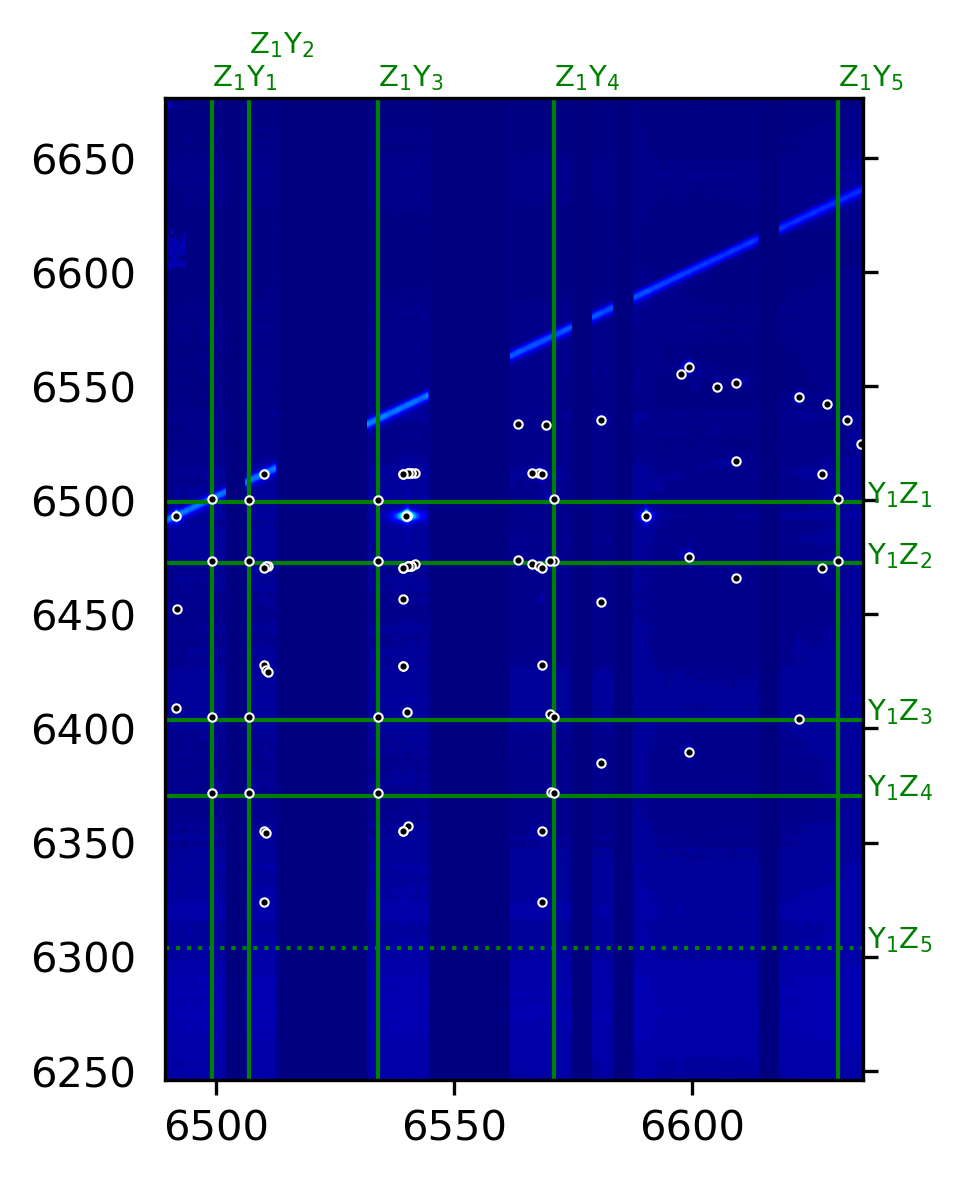
\includegraphics[scale=0.97]{JinD_site1_13K}\hfill
%   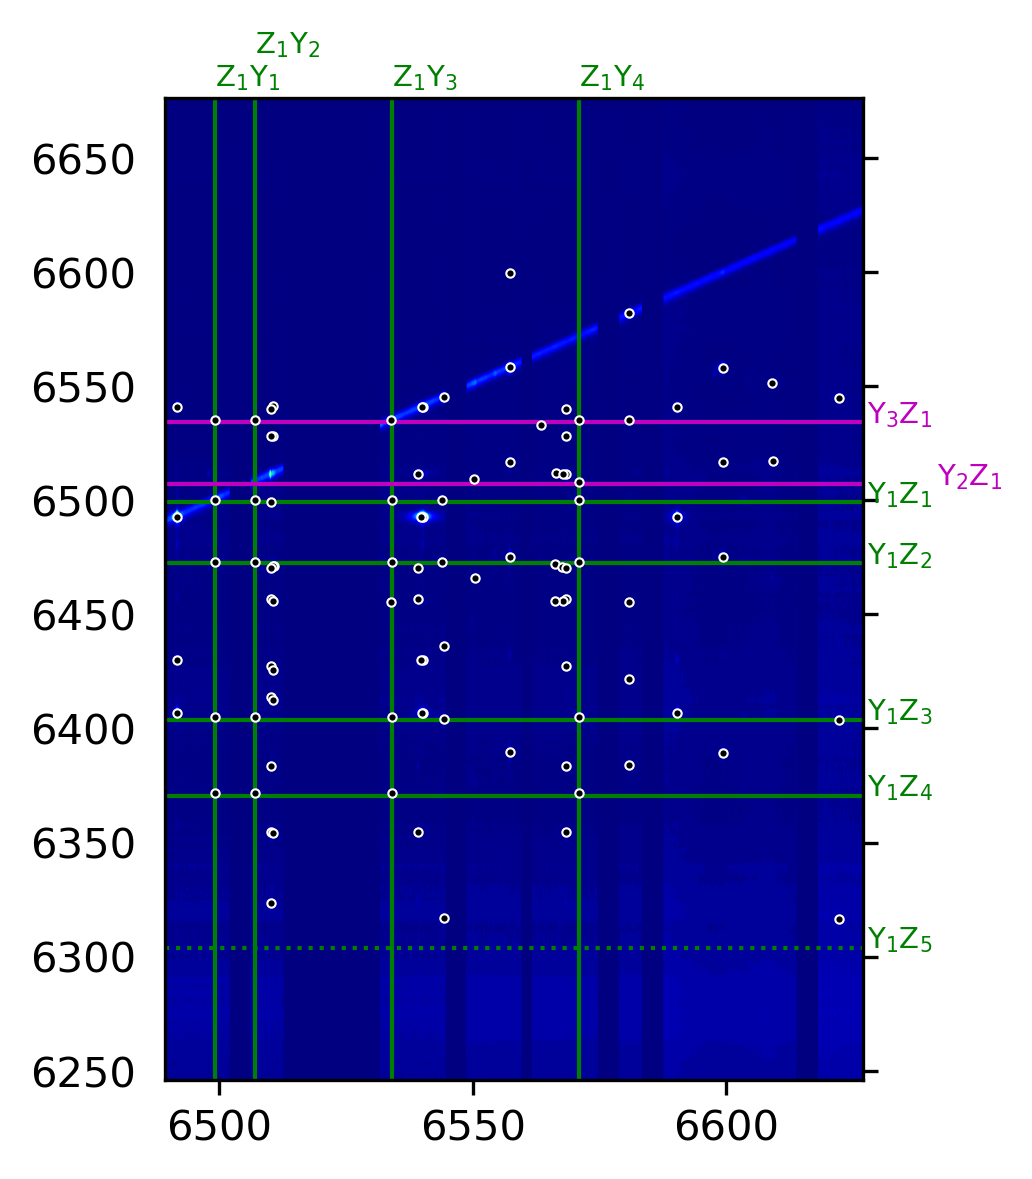
\includegraphics[scale=0.97]{JinD_site1_32K}\\
%   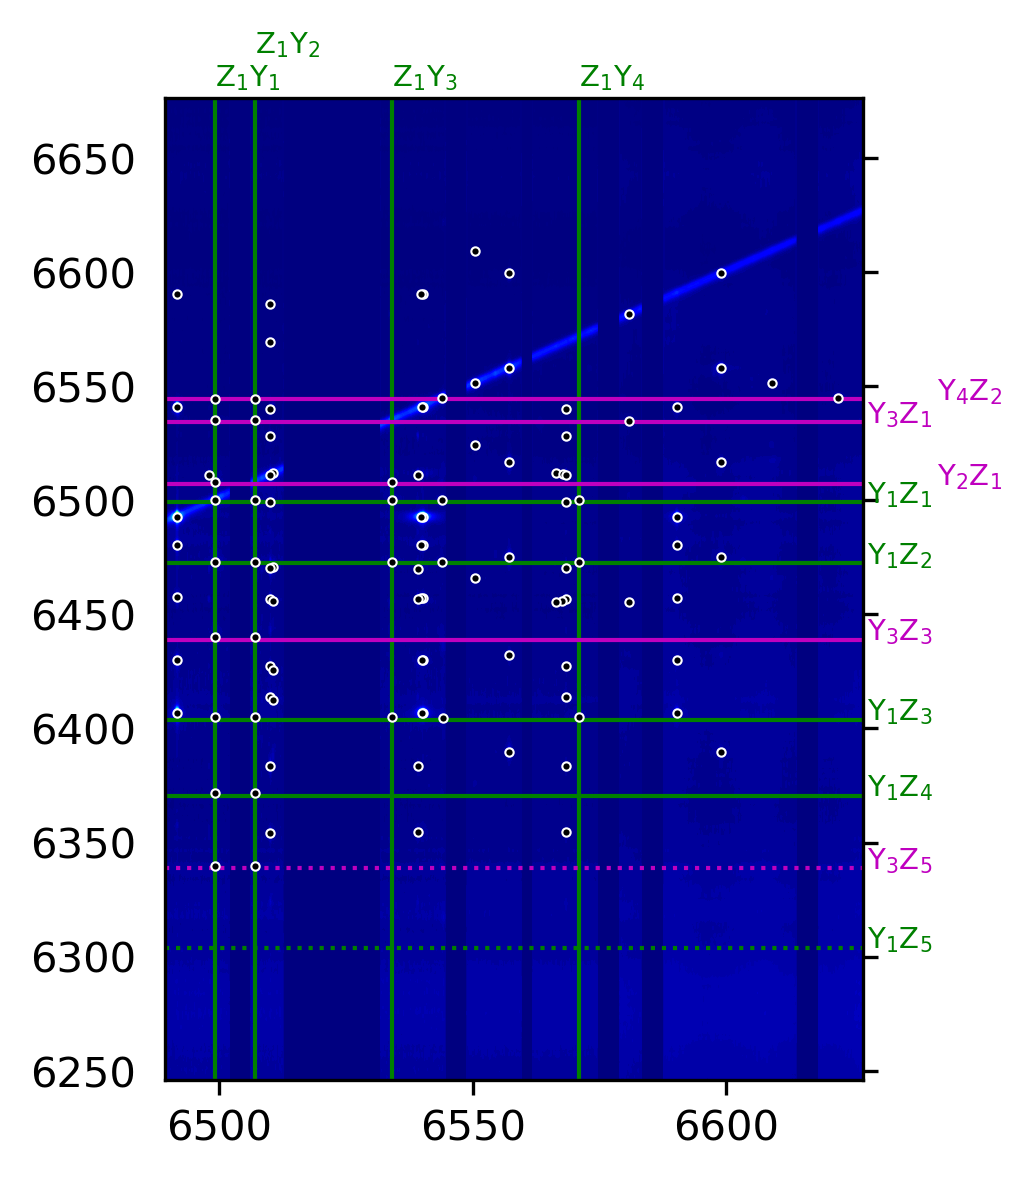
\includegraphics[scale=0.97]{JinD_site1_60K}\hfill
%   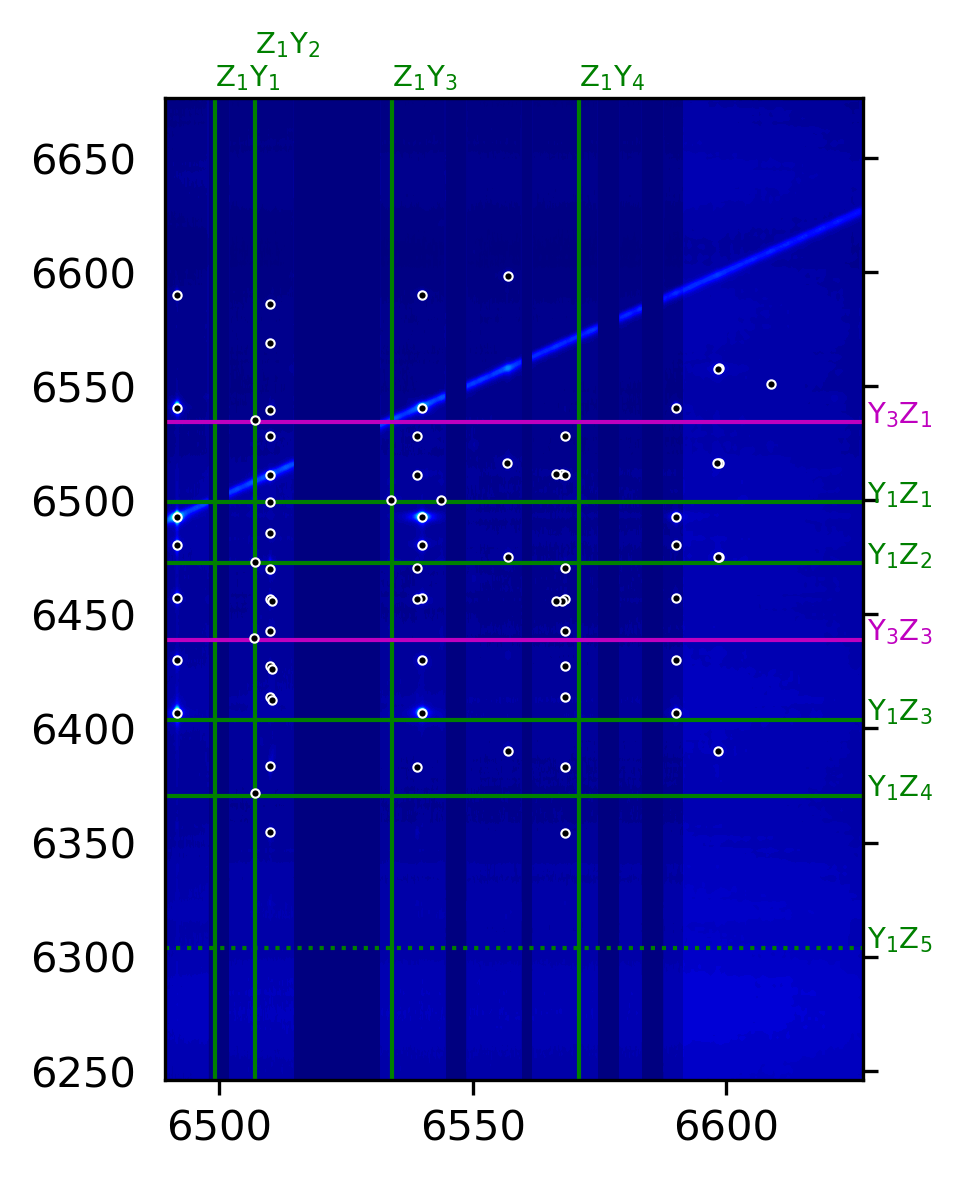
\includegraphics[scale=0.97]{JinD_site1_106K}
%   \caption{Transition assignments for excitation-emission spectra of MgO for Site 1 at 13, 32, 60, and 106K respectively. All observed peaks are marked. Green lines correspond to excitation (emission) from $Z_{1}$ ($Y_{1}$), magenta lines correspond to origin states that thermally occupy at higher temperatures.}
%   \label{fig:mgosite1}
% \end{figure}

% \begin{figure}[b]
%   \centering
%   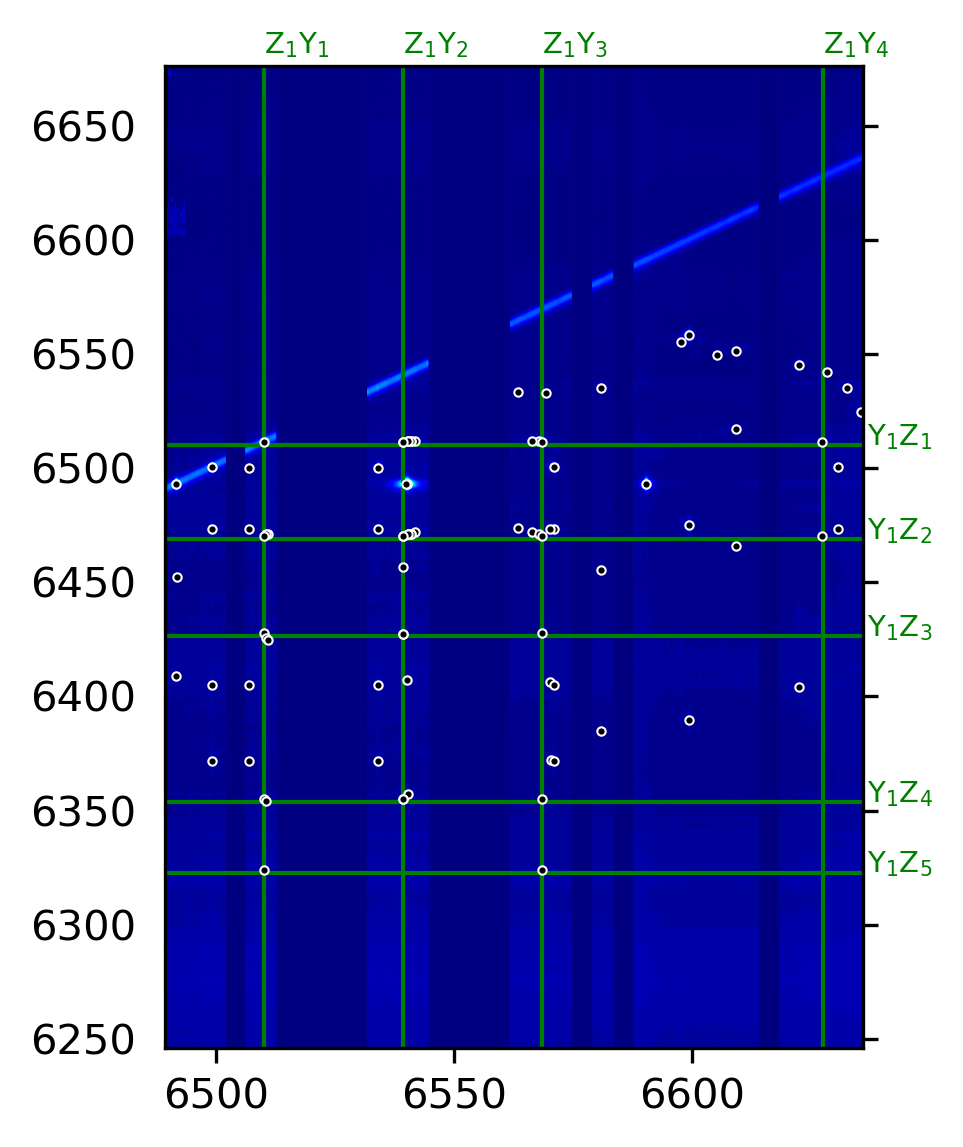
\includegraphics[scale=0.97]{JinD_site2_13K}\hfill
%   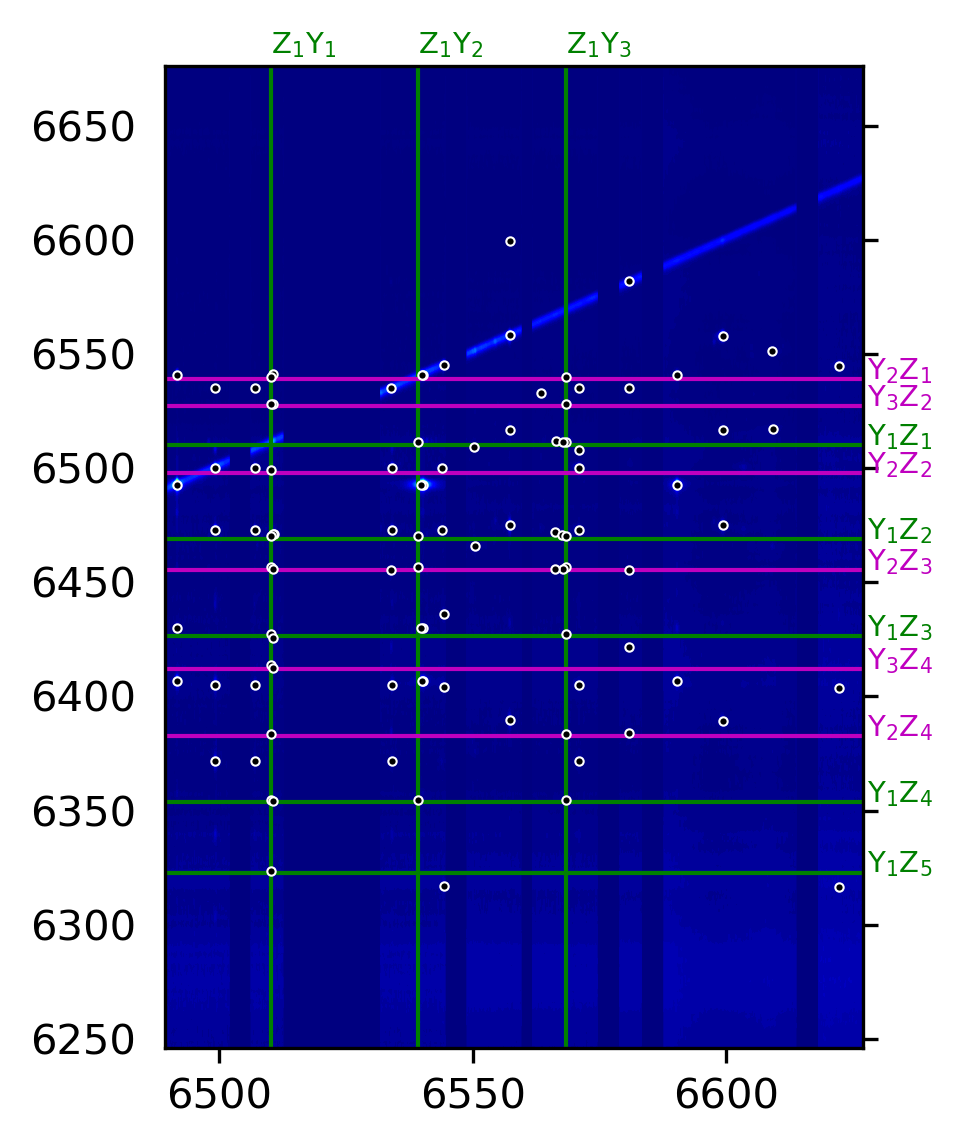
\includegraphics[scale=0.97]{JinD_site2_32K}\\
%   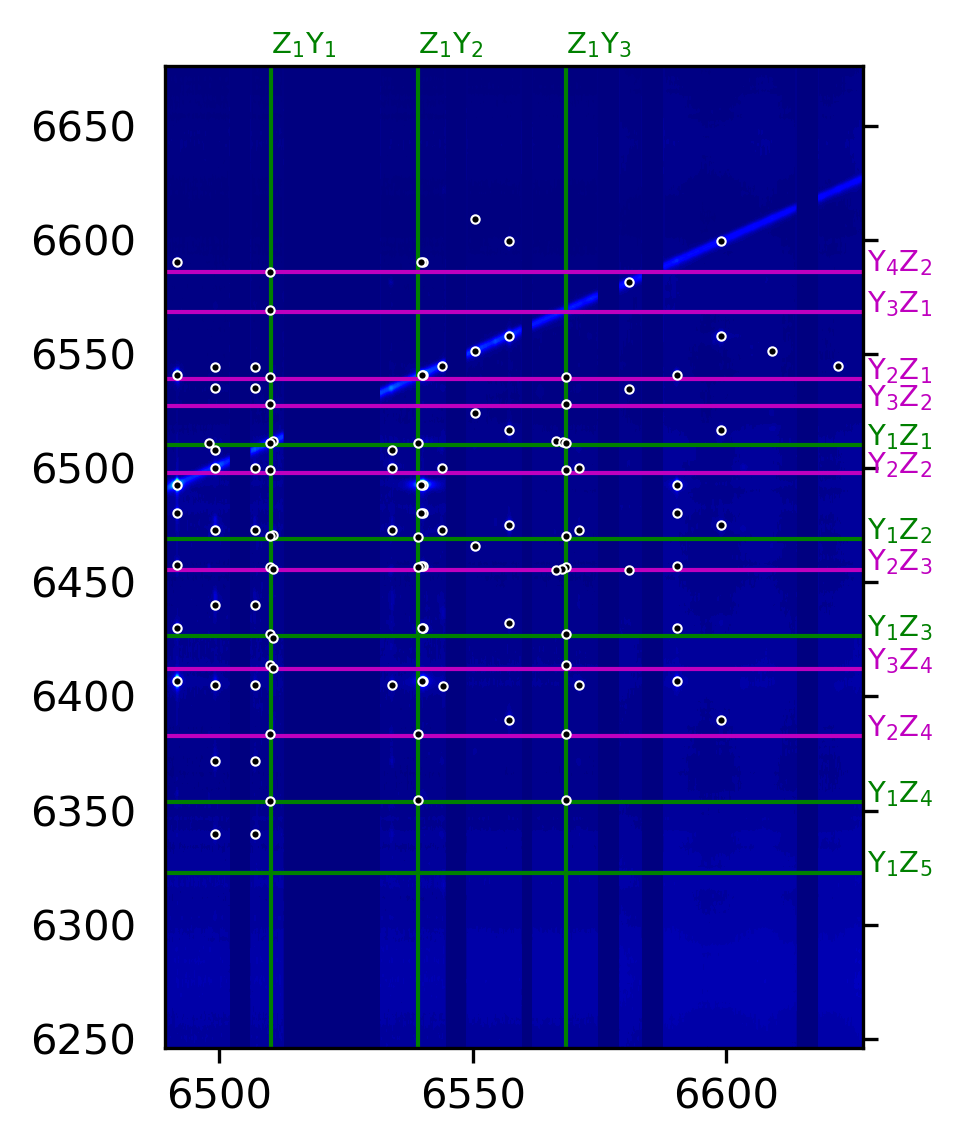
\includegraphics[scale=0.97]{JinD_site2_60K}\hfill
%   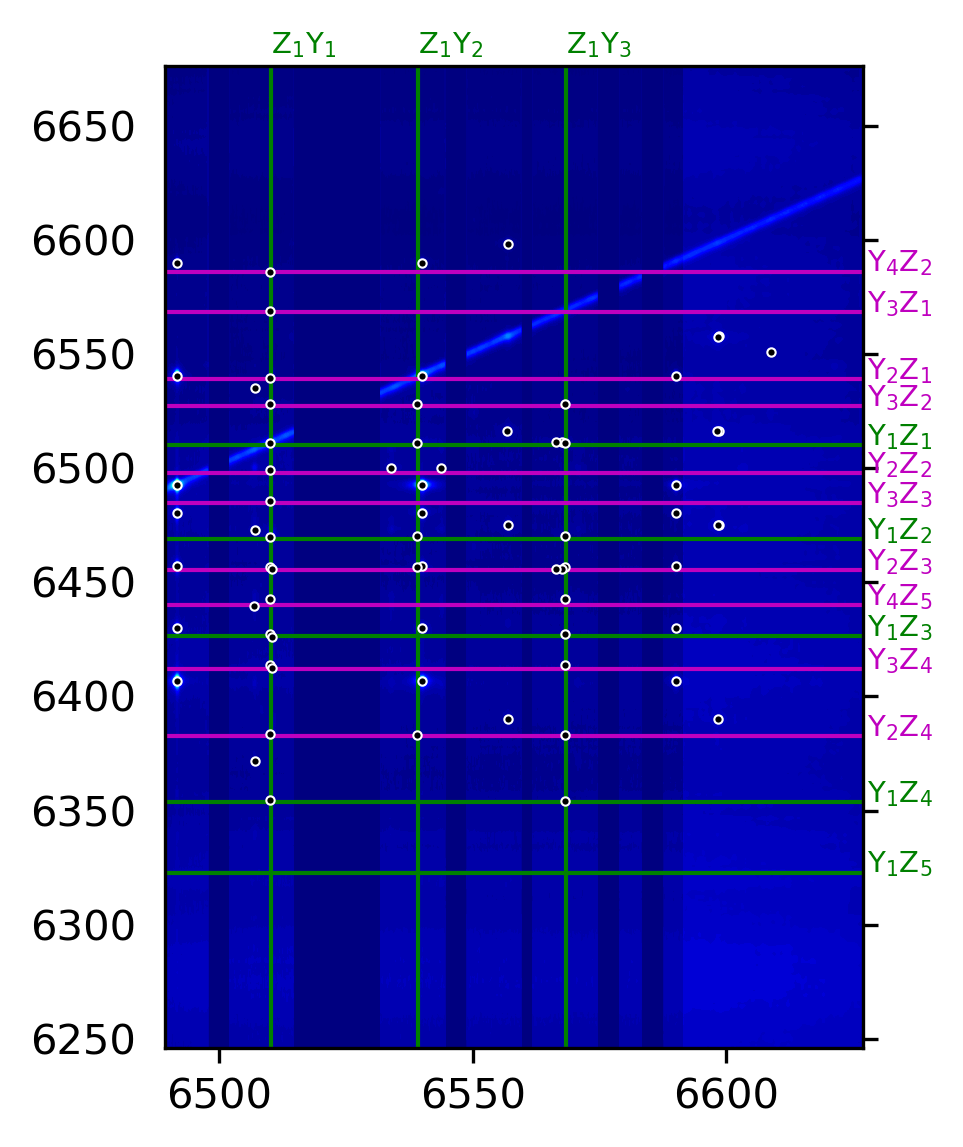
\includegraphics[scale=0.97]{JinD_site2_106K}
%   \caption{Transition assignments for excitation-emission spectra of MgO for Site 2 at 13, 32, 60, and 106K respectively. All observed peaks are marked. Green lines correspond to excitation (emission) from $Z_{1}$ ($Y_{1}$), magenta lines correspond to origin states that thermally occupy at higher temperatures.}
%   \label{fig:mgosite2}
% \end{figure}

% \begin{figure}[b]
%   \centering
%   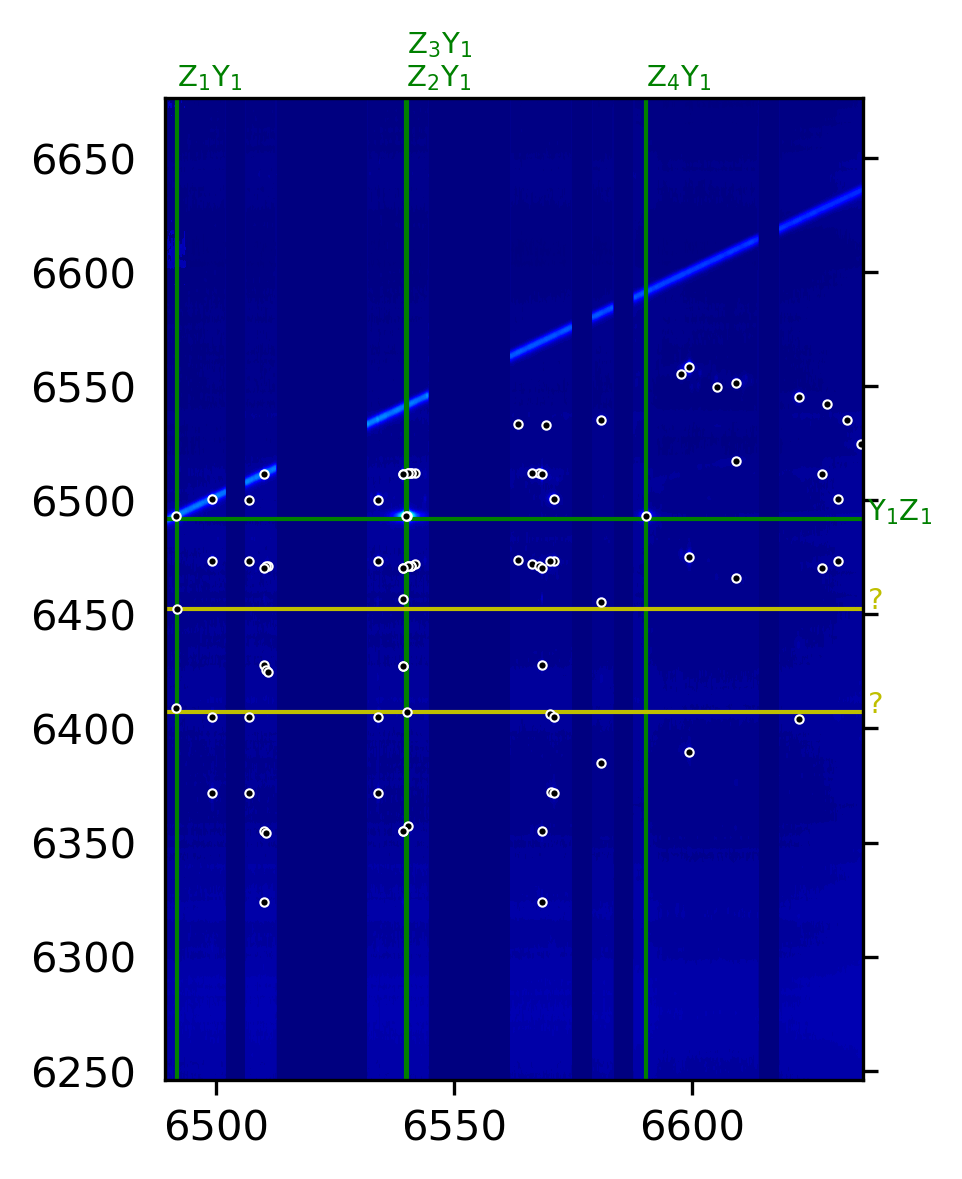
\includegraphics[scale=0.97]{JinD_site3_13K}\hfill
%   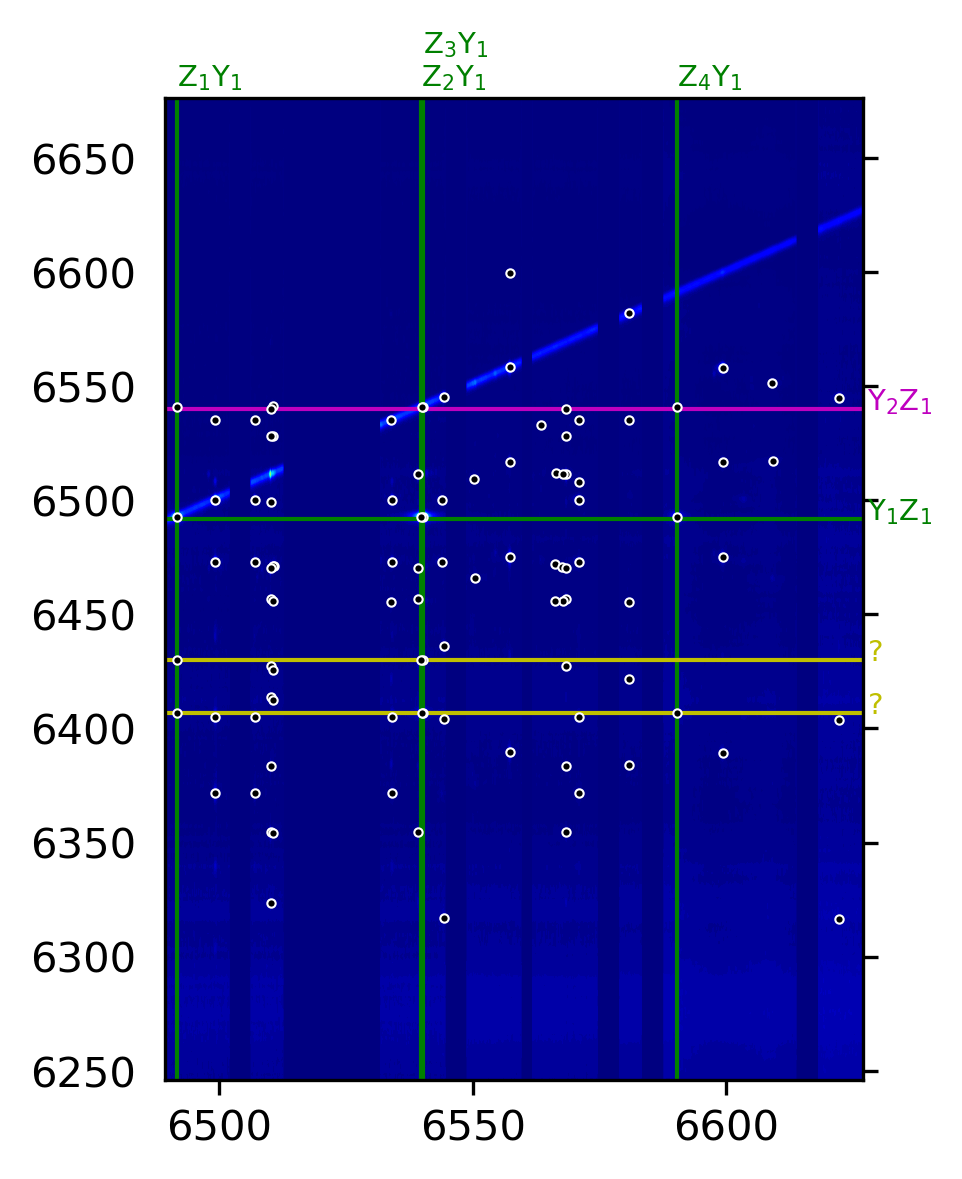
\includegraphics[scale=0.97]{JinD_site3_32K}\\
%   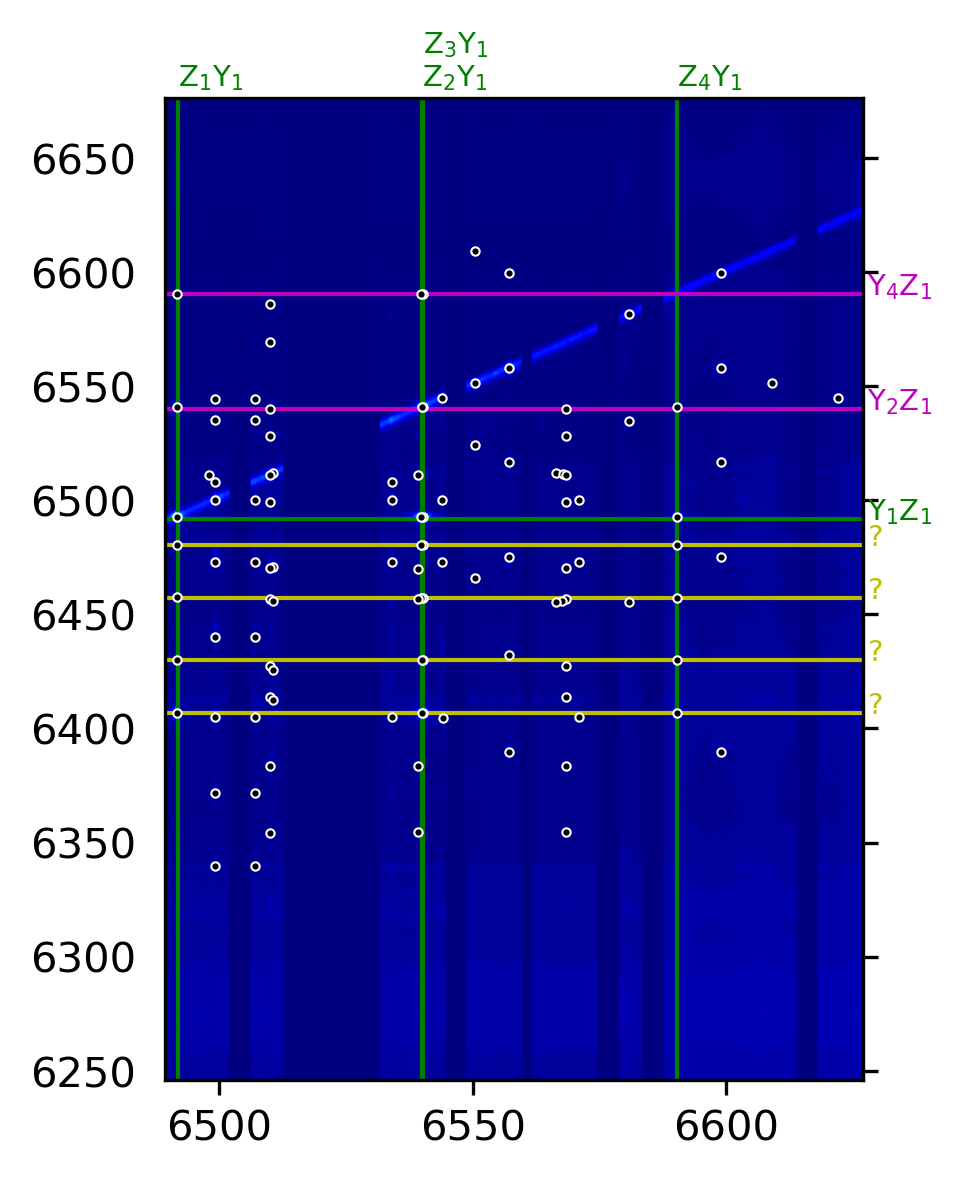
\includegraphics[scale=0.97]{JinD_site3_60K}\hfill
%   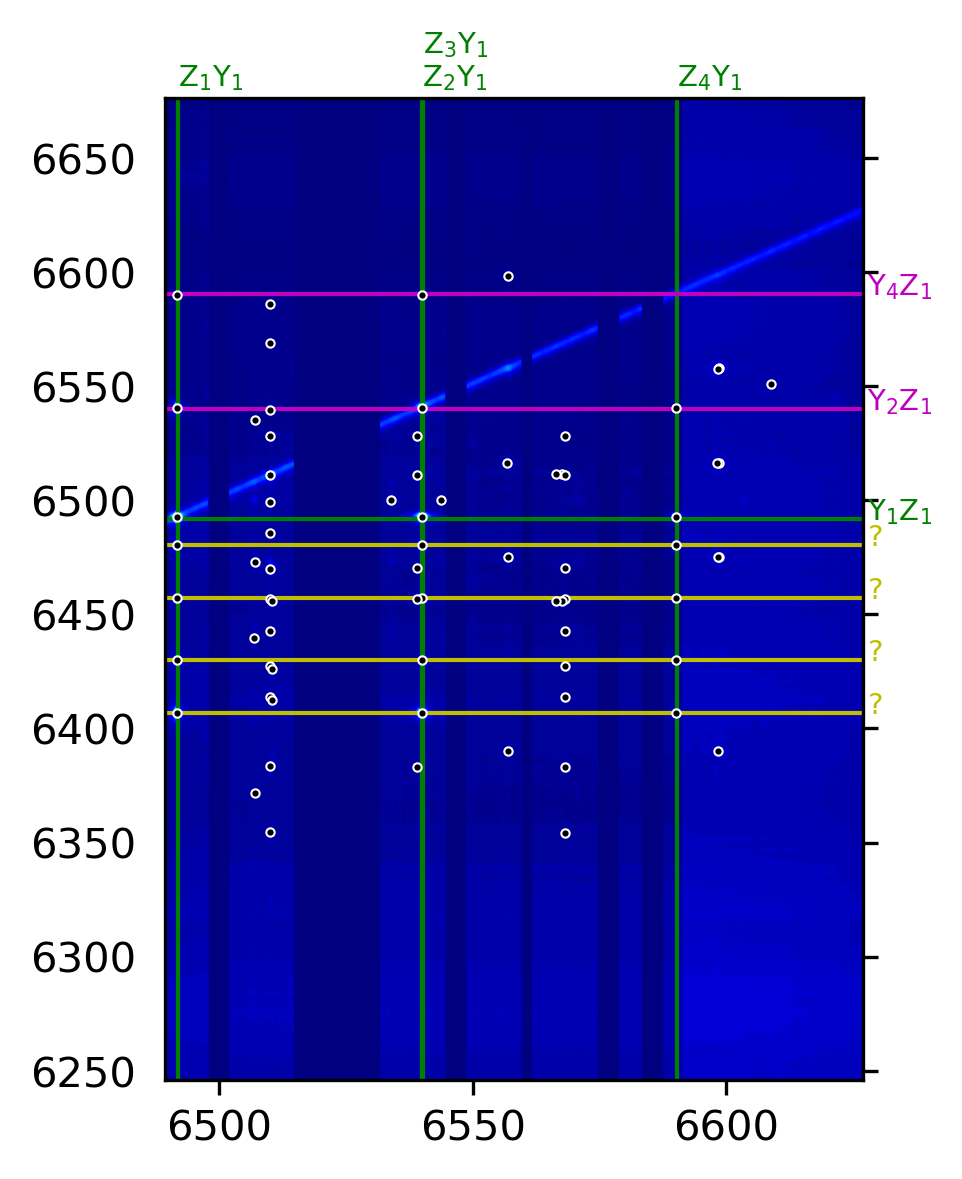
\includegraphics[scale=0.97]{JinD_site3_106K}
%   \caption{Transition assignments for excitation-emission spectra of MgO for Site 3 at 13, 32, 60, and 106K respectively. All observed peaks are marked. Green lines correspond to excitation (emission) from $Z_{1}$ ($Y_{1}$), magenta lines correspond to origin states that thermally occupy at higher temperatures. Emission lines for which no level assignment can be determined are plotted in yellow.}
%   \label{fig:mgosite3}
% \end{figure}

% \begin{figure}[b]
%   \centering
%   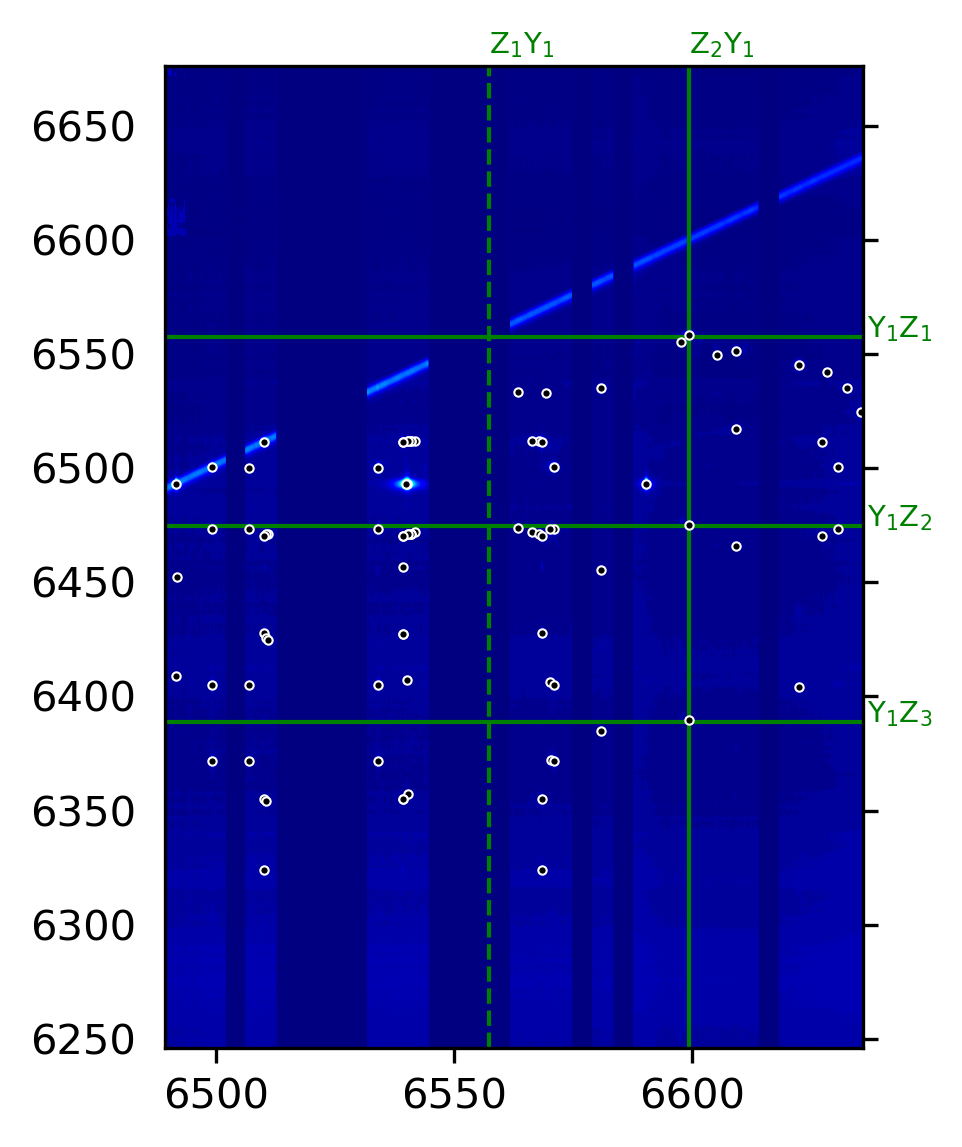
\includegraphics[scale=0.97]{JinD_site4_13K}\hfill
%   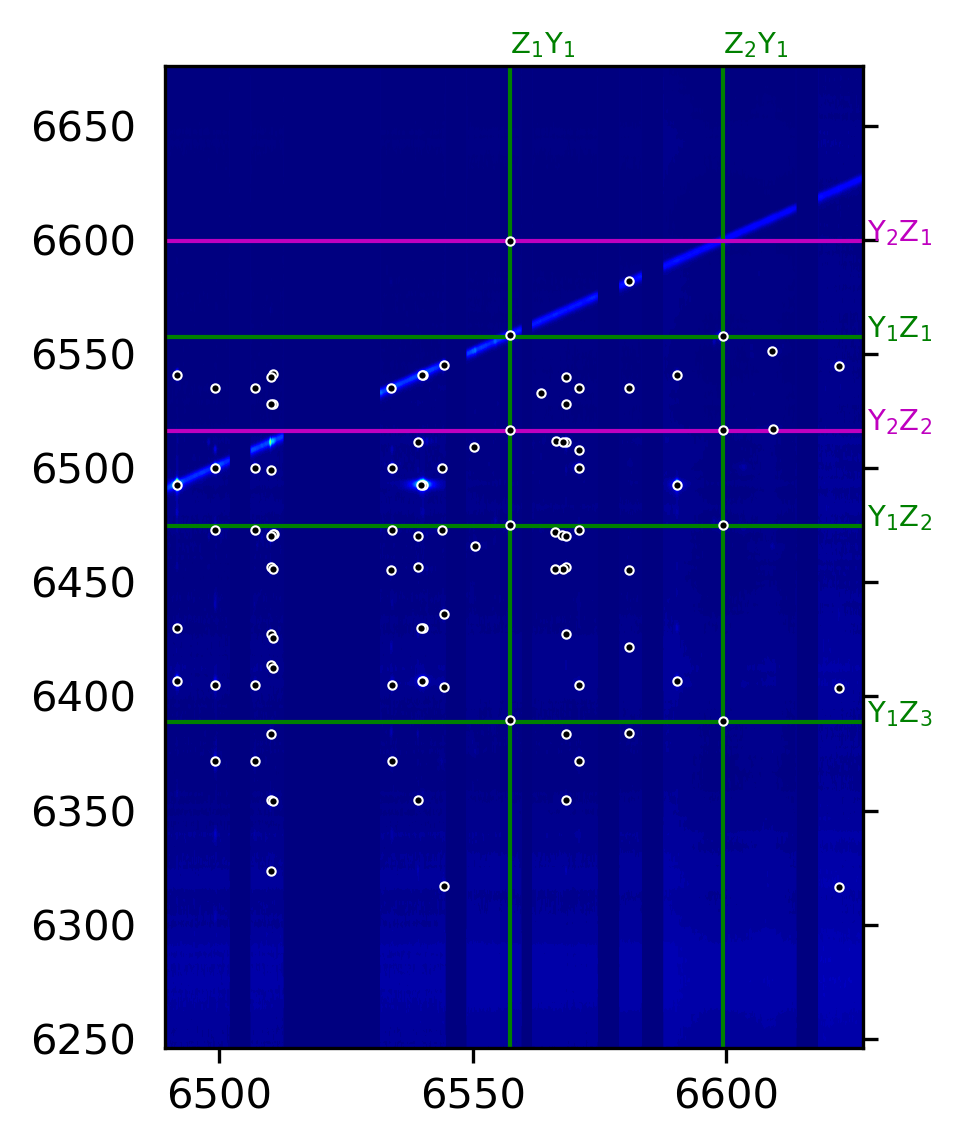
\includegraphics[scale=0.97]{JinD_site4_32K}\\
%   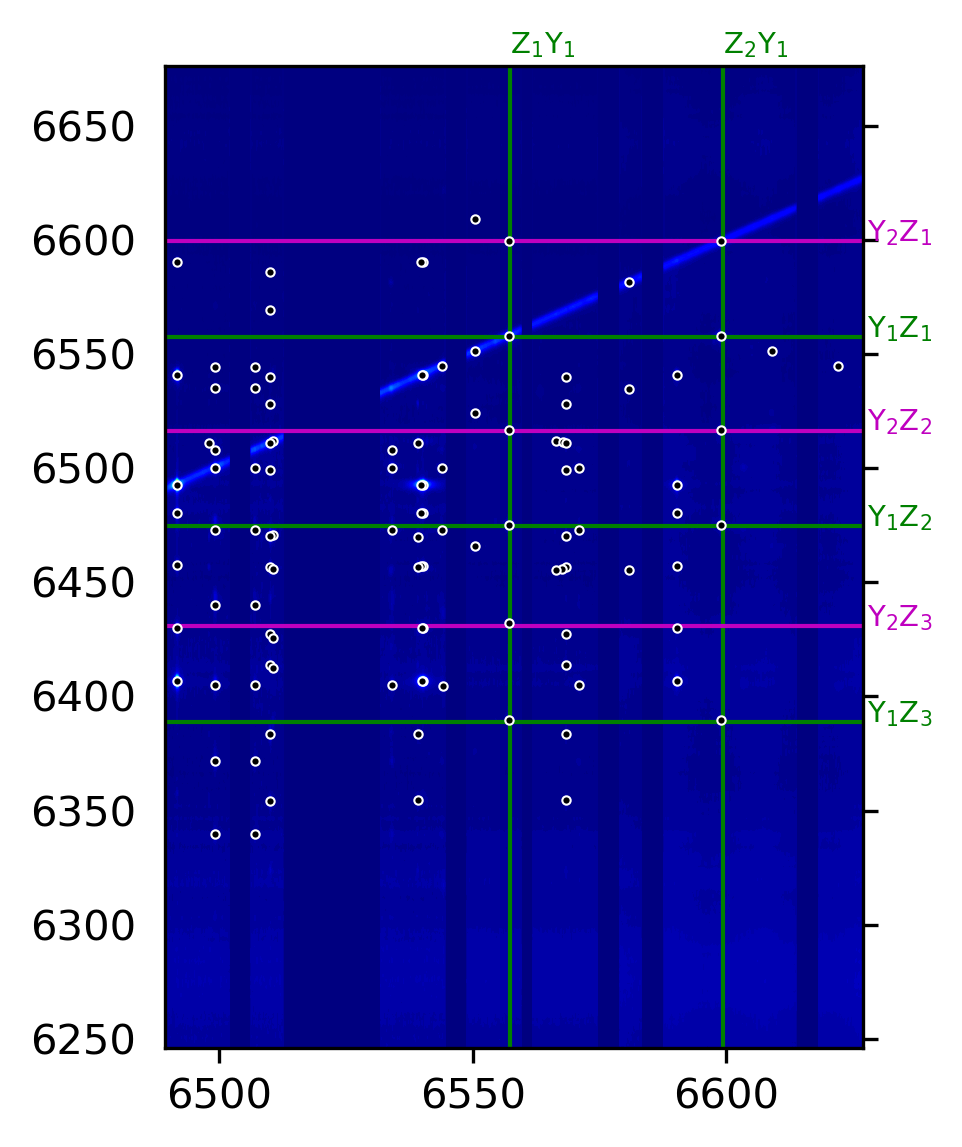
\includegraphics[scale=0.97]{JinD_site4_60K}\hfill
%   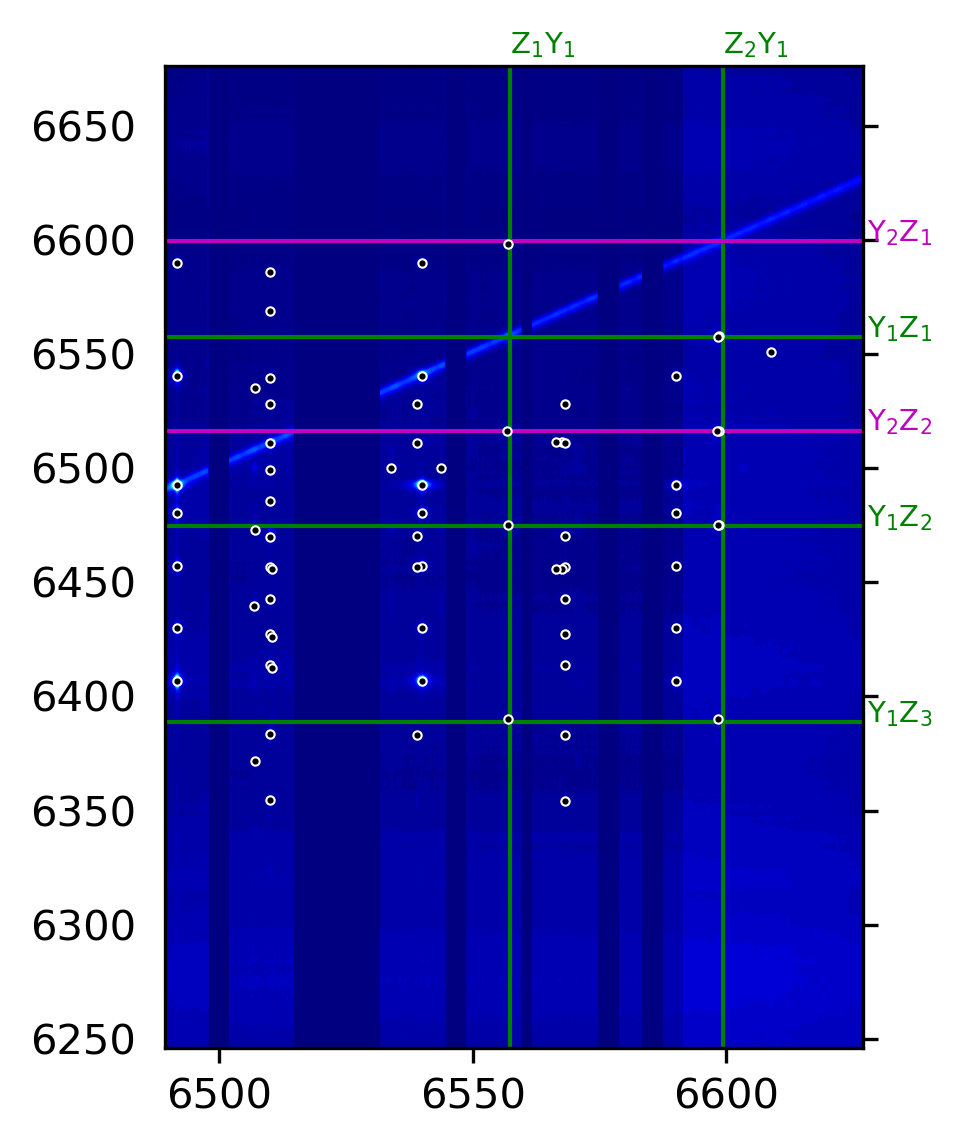
\includegraphics[scale=0.97]{JinD_site4_106K}
%   \caption{Transition assignments for excitation-emission spectra of MgO for Site 4 at 13, 32, 60, and 106K respectively. No data exists for $Z_{1}Y_{1}$ at 13K, so this line is dotted in that figure. All observed peaks are marked. Green lines correspond to excitation (emission) from $Z_{1}$ ($Y_{1}$), magenta lines correspond to origin states that thermally occupy at higher temperatures.}
%   \label{fig:mgosite4}
% \end{figure}

% \begin{figure}[t]
%   \centering
%   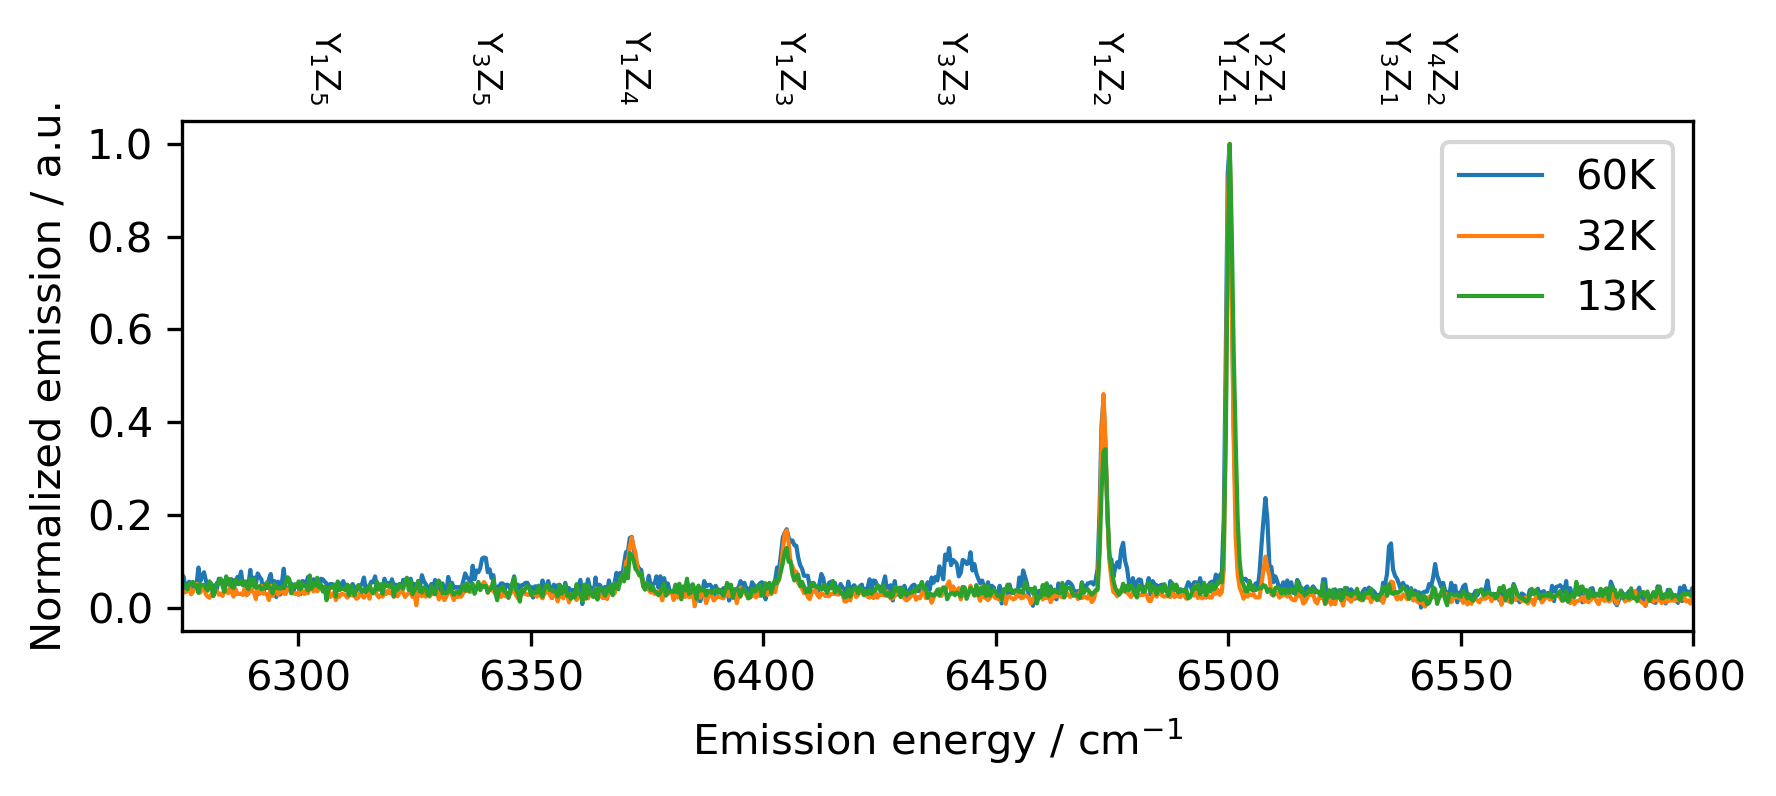
\includegraphics[scale=0.75]{JinD_site1_temp}
%   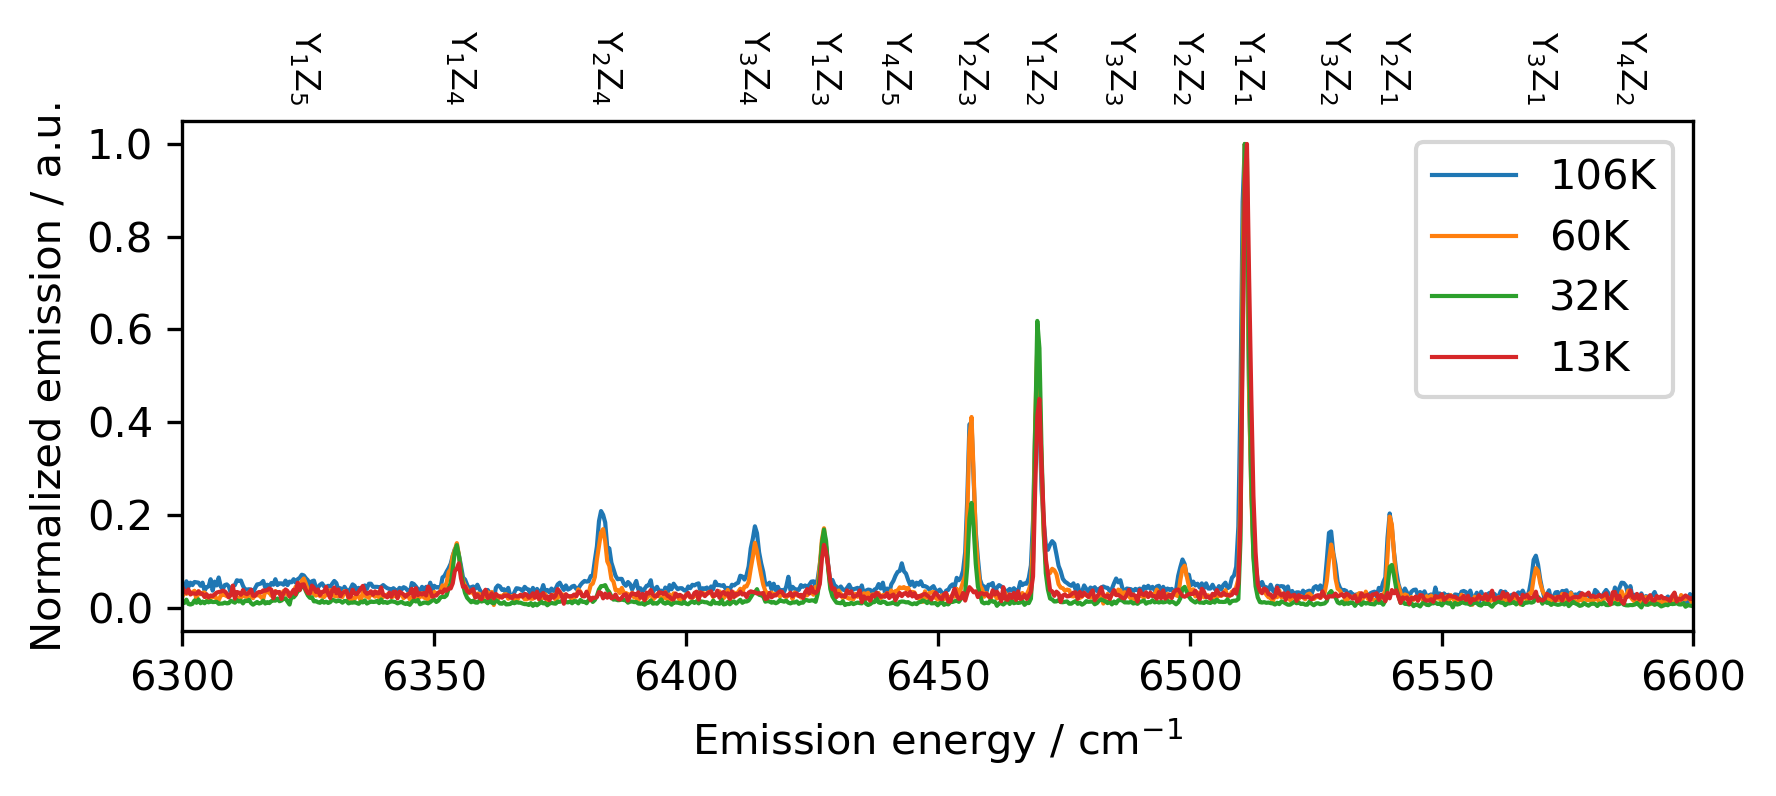
\includegraphics[scale=0.75]{JinD_site2_temp}
%   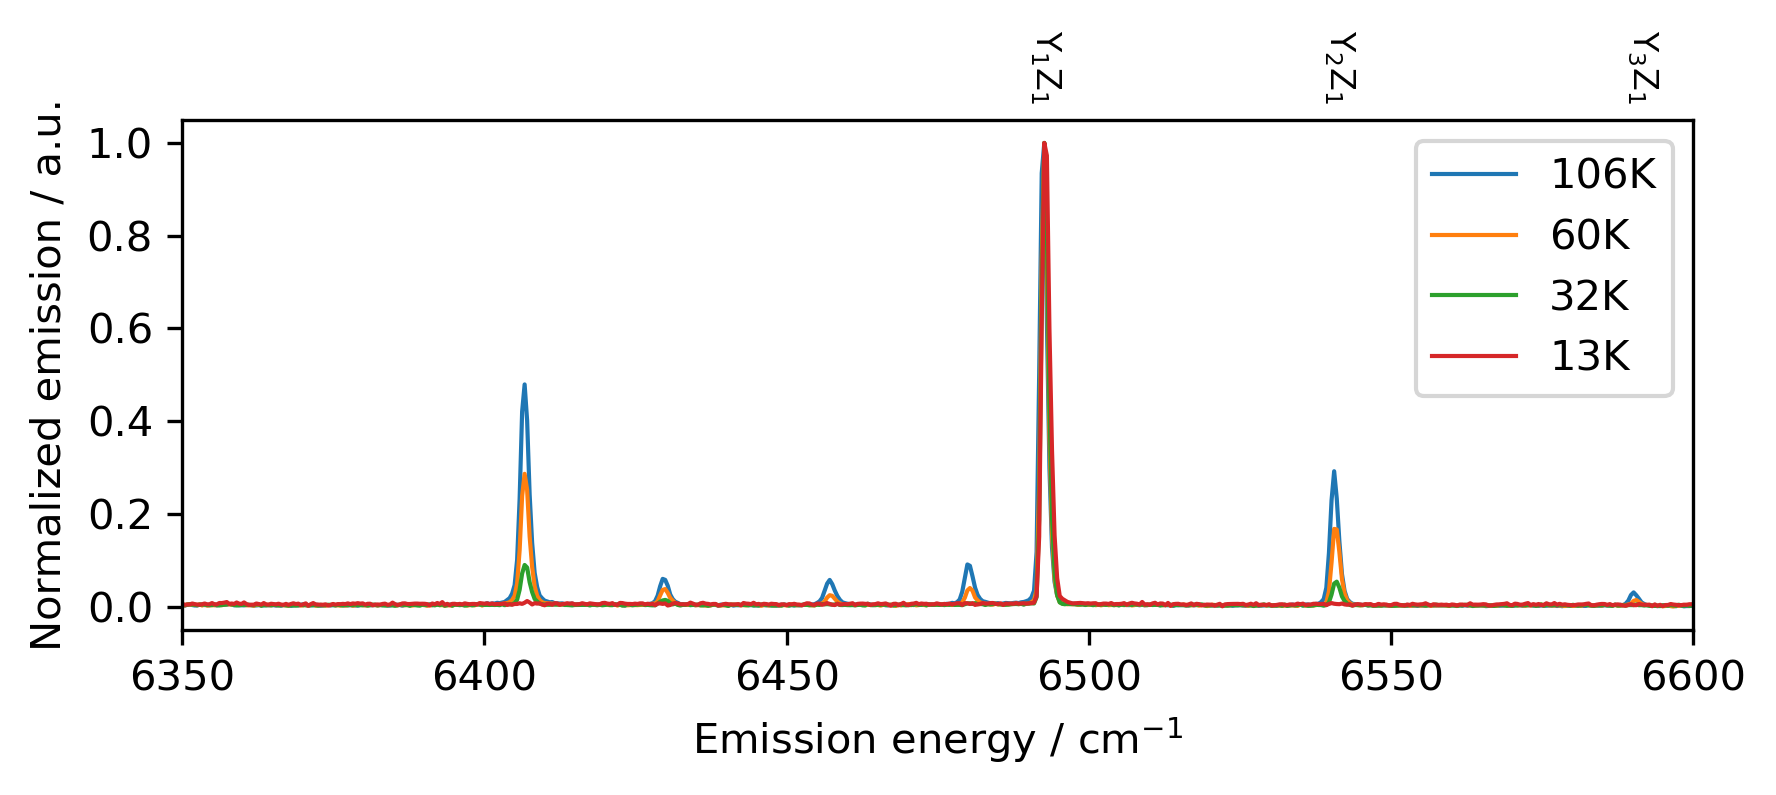
\includegraphics[scale=0.75]{JinD_site3_temp}
%   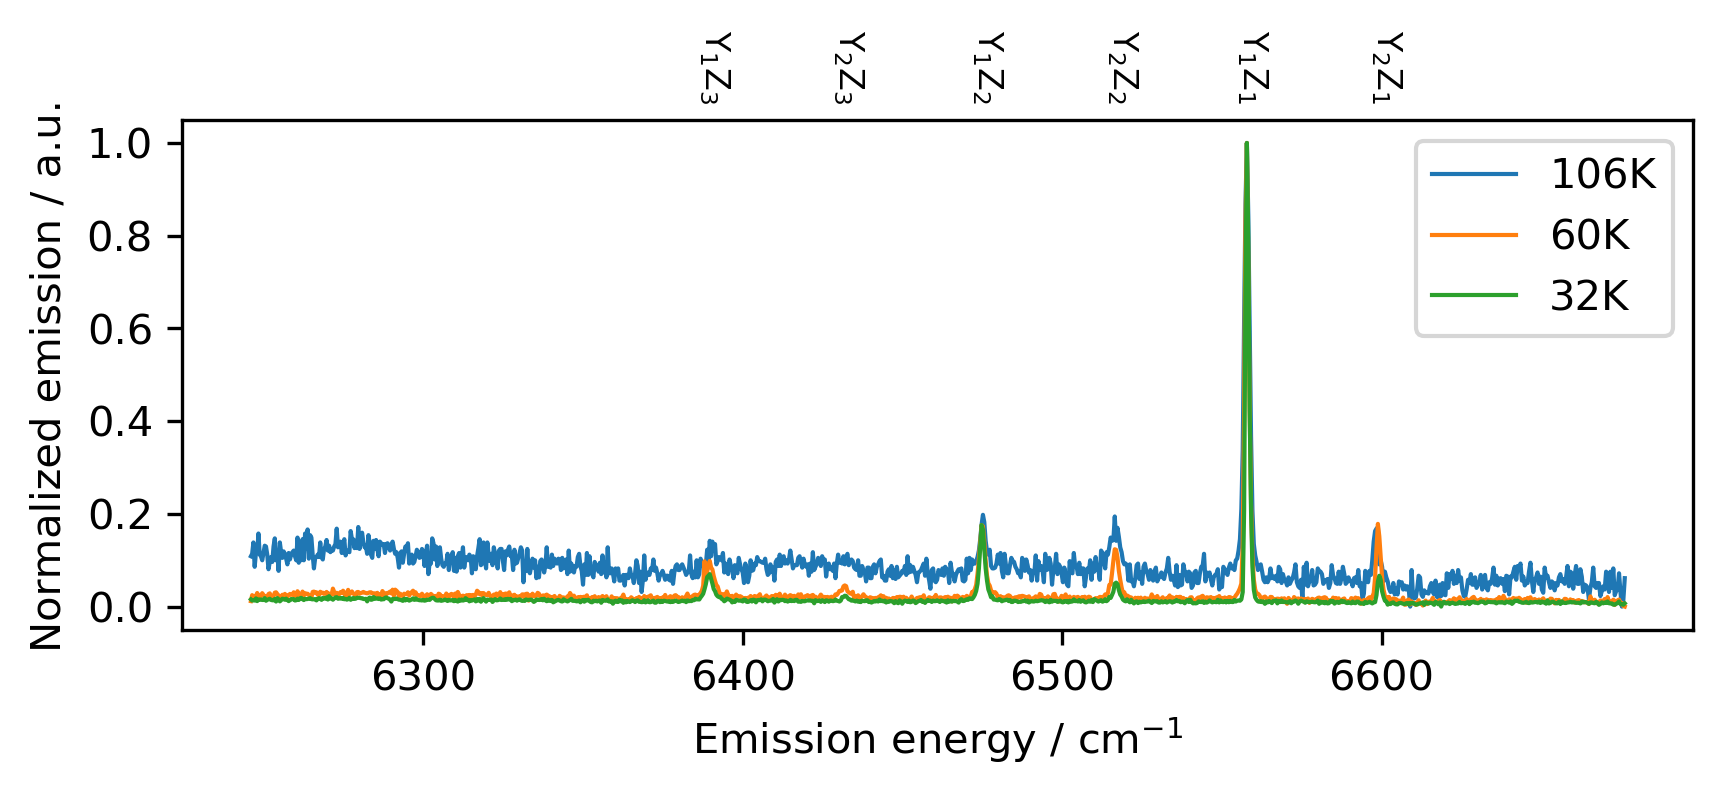
\includegraphics[scale=0.75]{JinD_site4_temp}
%   \caption{Temperature dependence of emission spectrum in MgO, excited at $Z_{1}Y_{1}$, for Sites 1, 2, 3, and 4, from top to bottom. Each peak is labeled with its corresponding emission transition.}
%   \label{fig:mgotemp}
% \end{figure}


%%%%%%%%%%%%%%%%%%%%%%%%%%%%%%%%%%%%%%%%%%%%%%%%%%%%%%%%%%%%

\chapter{Design of a low-cost, high-resolution Fourier transform spectrometer}

\section{Motivation}

The array-detector-based emission spectrometer greatly sped up the acquisition of excitation-emission spectra. However, it has two primary limitations which impose constraints on our measurements. One is the resolution. The detector has \notetoself{1024} bins, which sets the resolution on a 100 nm wide scan to only 0.1 nm, which is often not enough for our purposes. Furthermore, increasing the resolution by decreasing the width of the slit attenuates the signal, further lowering the signal to noise ratio.

The other limitation is the signal to noise ratio itself, which is not high enough for us to see all the peaks we might be able to see with a less noisy detection scheme. For the array detector, there are three main sources of noise. One is the readout noise of the detectors, which contributes roughly 700 counts per bin per readout operation and thus a constant noise level of roughly 25 counts per bin per readout. Another is leakage, both from the room and from the excitation light, which cannot be completely filtered out of the detector. And the third is dark counts in the detector, which correspond to the black box thermal photons inside the detector. Because of the readout noise, you can improve your measurement somewhat by acquiring data for a longer time; however, due to the dark counts and bleedthrough which occur at a constant rate in time, the signal to noise ratio eventually begins to plateau and your measurement stops improving substantially with longer acquisition times. Furthermore, the bins fill up after roughly 7000 counts, putting a further limit on the maximum acquisition time per readout.

The signal to noise ratio on the low-noise photodiode used for PLE is better than the signal to noise ratio on the array detector for the purposes of detecting the smallest signals possible. In part this is because a single detector simply introduces less noise than 1024 detectors. This has inspired the idea of using another of these low-noise photodiodes to build a Fourier transform spectrometer. This could provide several benefits over the current setup, including increased range and resolution, a higher signal to noise ratio, and no more need to focus through a slit. Additionally, if this technology is effective, the excitation source could be switched to a broad spectrum white light source and fed through a different Fourier transform setup, enabling study of a wider range of excitation wavelengths as well. 

\section{Principles of Fourier transform spectroscopy}

\begin{wrapfigure}{r}{0.3\textwidth}
  \centering
  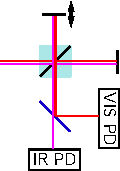
\includegraphics[width=0.23\textwidth]{FTIRMainIdea}
  \caption{A Fourier transform spectrometer.}
  \label{fig:ftirmainidea}
\end{wrapfigure}

The basic idea of a Fourier transform infrared spectrometer is depicted in Figure \ref{fig:ftirmainidea}. The infrared signal (magenta) is fed into a Michelson interferometer with one moving arm which sweeps back and forth, causing interference fringes. A different, narrow-linewidth laser in the visible spectrum (red) is fed in along the same beampath, and separated from the IR signal with a dichroic (blue). One detector measured the fringes in the visible spectrum reference laser, which are used to determine the position of the moving mirror at all time points. The IR signal coming out of the interferometer is measured simultaneously. Using the positions calculated from the red laser as the position axis, this signal is Fourier transformed into the spatial frequency domain. The frequency composition of the IR signal can thus be measured. 

The range and resolution of a FTIR spectrometer are deterined by physical properties of the system. The maximum measureable frequency is determined by the reference laser. The resolution is determined by the travel of the mirror. For two frequencies $\nu$ and $\nu+\delta\nu$ to be resolvable, the number of fringes you observe over the full travel of the mirror $L$ must be different by at least one, $N$ and $N+1$. Thus 
\begin{equation}\label{eq:9}
\delta \nu = \frac{1}{L}.
\end{equation}
So to achieve a frequency resolution of, for example, $1$ \wn\ we need the mirror to travel at least $1$ cm.

Different types of noise are treated differently in FTIR spectroscopy. White noise, like dark counts in the detector, simply becomes white noise again in the Fourier domain. Bleedthrough from other parts of the experiment or the room are treated differently depending on how they enter the detector. If they enter the multi-mode signal fiber, they are Fourier transformed along with the signal. If they scatter randomly into the detector, however, they become white noise as well in the Fourier domain.

The maximum scan speed is tied to the sampling rate of the detection scheme. In order to resolve the fringes of the reference laser, the speed of the mirror's travel must be limited so that the frequency of reference fringes in time (given by the mirror speed divided by the reference wavelength) is below the Nyquist frequency of the detector, i.e. one half of the sample rate.

The quality of the interferometer is tied to the signal to noise ratio of the spectrometer. The quality of the intereferometer is referred to as the ``contrast,'' and is measured as the peak-to-peak power variation of a narrow-linewidth coherent laser input divided by the total laser power at the detector (determined by blocking one arm of the interferometer, then the other, and adding the observed powers together).

When taking the discrete Fourier transform of the signal, it is desirable to first multiply the signal by a window, like the Hann window,\footnote{The Hann window is a consine centered on the middle of the signal with a wavelength of the entire spatial domain. It is thus zero at the edges of the domain.} which reduces the contributions of the edges of the spatial domain signal. There are two reasons for this. One is that the DFT assumes that the signal obeys periodic boundary conditions, which in our case it does not; thus, reducing the contributions of the boundaries to zero helps us by enforcing periodic boundary conditions. The other is that the motion of the mirror is slower near the turning points at the boundaries, and the data from these regions are thus of lower resolution and quality than the data near the center of the scan. It is therefore altogether fitting and proper that we reduce the contributions of the signal near the edges of the domain.

\section{Implementation}

An optical diagram of our FTIR spectrometer is given in Figure \ref{fig:ftirdiagram}. Both the reference laser (a HeNe laser at 633 nm) and the infrared signal are fiber coupled, and enter the setup through fiber collimators which are configured to focus as far away as possible (measured against the wall of the lab roughly 5 meters away). The beams are combined on a 1400 nm long-pass filter (LPF1). Rotation mounts on the fiber collimators, the subsequent IR mirror (M1), and the LPF allow the beam paths to be combined to high precision. This alignment was performed by placing an iris in the place of the removable mirror (M5), passing the beams through it, and aligning them in the far field. Accuracy was ensured by placing a beamsplitter immediately after the iris to ensure the power passing through the iris was maximal. This alignment ensures that the angular alignment of the two beams is within $\sim 0.1\%$.

\begin{figure}[b]
  \centering
  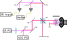
\includegraphics[width=\textwidth]{FTIRSetupDiagram}
  \caption{The optical design of our FTIR spectrometry setup. 1400 nm long-pass filters are marked in blue. A removable mirror is marked by a dotted line; when the mirror is taken out, the beams travel 3 meters to an alignment mark in the far field. }
  \label{fig:ftirdiagram}
\end{figure}

Next, the combined beams pass through a 50:50 beamsplitter (BS). One arm of the beamsplitter consists of a single mirror (M3) which return the beam along its original path. The other arm of the beamsplitter consists of a corner cube reflector attached to a speaker cone. The corner cube returns the incoming beam along a beampath parallel to the incoming beam regardless of orientation, which makes the interferometer relatively insensitive to slight rotations of the corner cube as the speaker cone moves in and out. The parallel beam is then reflected off another mirror (M4) and returns along the original path to be interfered with the M3 beam at the beamsplitter. Because the beam passes through the corner cube twice, the total beam path displacement is four times the travel of the corner cube, increasing the resolution by a factor of two over schemes where the beam only reflects off the moving surface once.

The alignment of the moving arm of the interferometer is performed by removing the removable mirror M5, and adjusting the rotation of M4 until the beams from the two arms are aligned in the far field. If the alignment is good, flickering will be visible. Next, the mirror M5 is replaced, and the different frequencies of light are focused onto their respective detectors after being separated by another long pass filter (LPF2). The alignment of M4 is refined by sweeping the speaker to generate fringes, then maximizing the contrast of the fringes on the reference detector.

Next, the path lengths of the two arms of the interferometer must be equalized so that the zero path length point occurs in the middle of each sweep of the moving arm. For this step, a fiber-coupled infrared LED with a linewidth of tens of nanometers is used as an input to the infrared side of the interferometer. The Fourier transform of this signal is roughly a sine wave multiplied by an envelope whose width is inversely related to the linewidth of the signal. Since the width of this envelope is on the order of half a millimeter, the zero path length point shows up in the swept IR signal as a narrow peak surrounded by flat background. The mirror M3 is then translated forward and backward on a translation stage until the zero path length point is located and centered in the scan.

At this point, the rotational alignment of the mirror M3 is adjusted to once again optimize contrast, as the translation stage introduces small angular displacements. After adjusting the lens in front of the infrared photodiode to maximize the signal, the setup is prepared for data acquisition.

To take a scan, the frequency on the function generator which powers the speaker is adjusted to the appropriate scan frequency (discussed further in Section \ref{sec:characterization}). The data acquisition device is configured to measure, at maximum sample rate, the output signal of both photodiodes and the synchronization pulse of the function generator. These outputs are recorded and saved.\footnote{In the future, data processing will be handled in real time to reduce file sizes.}

The data processing occurs in three steps. First, individual sweeps are separated from one another using the synchronization pulses from the function generator. Next, the samples are rebased from the time domain to the spatial domain. The zero crossing points of the reference signal are identified. The IR signal data between each zero crossing point and the next is averaged together, becoming a single data point on the new axis of spatially indexed data, where each point is separated from the next by half the reference wavelength (316.5 nm). Third and finally, this spatially indexed data is Fourier transformed using a Hann window into the spatial frequency domain. 

\section{Characterization}
\label{sec:characterization}

The first important characteristic of our FTIR setup is the maximum frequency at which the scans can be acquired. In our experiment, the signal from the photodiodes is read out by a National Instruments DAQ card whose sample rate is limited to 12500 samples per second, which is lower than the bandwidth of the photodiode; thus, the maximum speed of our measurements is limited by the sample rate. The scans must be performed slow enough that the fringes of the reference laser occur at a lower frequency than the Nyquist frequency of the detector, i.e. half the sampling frequency.

This sets an upper bound on the scan rate. By first driving the mirror as slow as possible and calculating the total displacement, the total number of fringes expected over the course of a scan was calculated. Then the mirror was driven at a frequency just low enough that at its maximum speed, the number of samples per fringe would be greater than one. This frequency was found to be $\sim 0.5$ Hz. Figure \ref{fig:reference} shows the reference signal at the fastest point in the mirrors travel, with the mirror being driven at 0.5 Hz. The number of fringes per sample is just below one, at roughly 0.85 (according to the fit). It is true, of course, that the nature of the Nyquist frequency is that higher frequency sine functions could also replicate this data; this is why we first drove the mirror well below the Nyquist frequency to calculate the rates.

\begin{figure}[t]
  \centering
  \includegraphics[scale=1]{RawRefSignal}
  \caption{Raw data (black) from the reference PD, taken from the center of the scan when the mirror is moving fastest. The mean of the data has been subtracted for clarity, and a cosine has been fitted to the data (red dotted line). The frequency of the fitted cosine is a factor of 0.85 below the Nyquist frequency.}
  \label{fig:reference}
\end{figure}

It is also worth noting that scanning slower than this determined rate of $0.5$ Hz is not advantageous. The discrete Fourier Transform (DFT) of a sine curve with frequency $\omega_{0}$, sampled at intervals of $\delta$, and with Gaussian distributed white noise $\eta(t)$, is 
\begin{equation}\label{eq:10}
\tilde f_{k} = \sum_{n=0}^{N-1}\left(\sin (\omega_{0}n\delta) +\eta(n\delta)\right)e^{-\frac{2\pi i}{N}nk}. 
\end{equation}
If we double the sampling rate, the new DFT is 
\begin{align}
  \tilde f'_{k}
  =& \sum_{n=0}^{2N-1}\Big(\sin(\omega_{0}n\delta/2) + \eta(n\delta/2)\Big)e^{-\frac{2\pi i}{2N}nk}\nonumber \\
  =& \sum_{n=0}^{N-1}\Big(\sin(\omega_{0}n\delta)+\eta(n\delta)\Big)e^{-\frac{2\pi i}{N}nk}\nonumber \\
  &+ \sum_{n=0}^{N-1}\Big(\sin\big(\omega_{0}(n+1/2)\delta\big) + \eta\big((n + 1/2)\delta\big) \Big)e^{-\frac{2\pi i}{N}(n+\frac{1}{2})k}.
  \label{eq:11}
\end{align}
After normalizing for the extra samples, we find that $f'$ is effectively the average of two completely separate scans at the original sampling frequency. The noise level thus decreases as the square root of the time taken, exactly the same as it would if several scans at the original scan rate were recorded. Thus, it is preferable to operate the scans as fast as the Nyquist frequency of the detector allows, and if averaging is necessary, to simply perform multiple independent scans rather than slow down the scan speed of a single scan. This is because the response of the speaker to being driven by the function generator becomes less reliable at lower frequencies.

\begin{wrapfigure}{r}{3.2in}
  \centering
  \includegraphics[scale=1]{Speed}
  \caption{Mirror displacements versus time at 0.5 Hz for two complete scans (one in each direction), with a fitted cosine.}
  \label{fig:speed}
\end{wrapfigure}

The next important characterization is to determine how far the mirror travels, and how smoothly. Figure \ref{fig:speed} shows the distance versus time curve for an example scan at 0.5 Hz. The distance is determined as the sum of the number of zero crossings of the reference signal, times half the reference wavelength. The inversion point at $\sim 2$ seconds was determined from the synchronization pulse. The good agreement between the data and cosine fit shows that the mirror travels smoothly on the speaker. It also shows tthat the scanning speed is sufficiently low, because if we started missing zero crossings near the fastest point in the scan the fit would not agree well anymore because our distance measurements would be inaccurate.

By extracting the maximum travel distance from the data in Figure \ref{fig:speed}, we find that the total beam path displacement over the course of a scan is $\sim 4.4$ mm. By equation \eqref{eq:9}, this gives us a potential frequency resolution of $\sim 2.3$ \wn[]. The frequency resolution of the array detector in its normal operating mode is $1.08 \pm 0.04$ \wn[]. This number was found by fitting Gaussian curves to the emission spectrum of the bleedthrough from the Toptica laser, as shown in Figure \ref{fig:emresolution}. Thus, for the resolution of the FTIR spectrometer to be comparable to the array detector, the travel needs to be increased by at least a factor of two.

\begin{figure}[t]
  \centering
  \includegraphics[scale=1]{EmissionResolution}
  \caption{Emission spectra of the Toptica bleedthrough at four different excitation points (selected for having no fluourescence) in an MgO excitation-emission spectrum recorded using the array detector. Data (black) have been fitted with Gaussian curves (red dotted lines), and the widths of the Gaussians extracted. The average width is $1.08\pm 0.04$ \wn[.]}
  \label{fig:emresolution}
\end{figure}

There are several potential ways to accomplish this. The first has to do with the electronics driving the speaker. The speaker has an impedance of 8 Ohms, and is rated to handle powers up to $25$ W. However, the function generator currently driving the speaker is only capable of outputting 200 mA, which corresponds to a voltage amplitude of $1.6$ V and a maximum power of only $0.32$ W. It therefore seems that we are not utilizing the full travel range of the speaker due to electronic limitations. Adding a current buffer to the output of the function generator could therefore increase the resolution of the FTIR spectrometer, potentially by up to an order of magnitude.

The second is optical, and involves reflecting the output beam through the corner cube a third and fourth time. This would double the effective travel of the corner cube, and could be accomplished by a scheme like the one depicted in Figure \ref{fig:newmirrorscheme}. Essentially, a second corner cube is arranged so as to reflect the beam back into the moving corner cube, at a displaced location, so that it passes through the moving corner cube a second time before being reflected back by the D mirror. While this scheme isn't easily extended beyond one iteration, it would double the resolution of the FTIR spectrometer, bringing it up to the resolution of the array detector spectrometer. 

\begin{figure}[t]
  \centering
  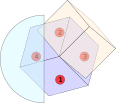
\includegraphics[width=0.43\textwidth]{NewMirrorScheme}
  \caption{A new corner cube mirror scheme to double the effective resolution of the spectrometer. The corner cube is being viewed head on from the perspective of the beamsplitter. The beam enters at point 1, and exits the mobile corner cube (purple) at point 2. It is then reflected off a second, stationary corner cube (orange) which faces the mobile corner cube, and is rotated so that the beam only reflects off two of the faces. The beam then reenters the mobile corner cube at point 3, and exits at point 4. It then reflects off a D-shaped mirror (mint) and returns to the beamsplitter along the same path, passing through points 4, 3, 2, and finally 1.}
  \label{fig:newmirrorscheme}
\end{figure}

The next characterization of the FTIR spectrometer we performed was on a broad spectrum signal from an infrared LED amplified by an EDFA. The results of this experiment are depicted in Figure \ref{fig:LED}. As expected, the raw signal is strongly enveloped around the zero path length point (the slight displacement is due to imperfect calibration). The spectrum shows a wide feature (roughly 150 \wn in total). This feature, examining the detail plot in the top right, appears to consist of a wide flat feature from 6400 to 6550 \wn[], and a taller, narrower feature from roughly 6500 to 6550 \wn[.] We suspect that this odd shape has to do with the amplification of the EDFA. Next, we would have measured this same spectrum using the array detector spectrometer to confirm the accuracy of the FTIR spectrum. Unfortunately, labs were shut down before this was possible. However, these results show that the FTIR spectrometer is at least minimally capable of measuring broad spectra. 

\begin{figure}[t]
  \centering
  \includegraphics[height=2.5in]{LEDsignal}
  \includegraphics[height=2.5in]{LEDspectrumzoom}
  \includegraphics[height=2.5in]{LEDspectrum}
  \caption{Top left: raw infrared photodiode signal for the broad spectrum LED. Bottom: complete power spectrum for the broad spectrum LED. Top right: detail plot of the boxed region in the bottom figure.}
  \label{fig:LED}
\end{figure}

Now tested on arbitrarily narrow signal. Findings:
SNR
FWHM
Accuracy
Important to discuss that this is cheap IR PD
Photon per second resolution?
2.00e+14 photons per second in toptica beam
What is proposed SNR gain with fance PD?


\begin{figure}[t]
  \centering
  \includegraphics{TOPspectrum}
  \caption{Detail plot of the only feature in the FTIR frequency spectrum of the Toptica diode laser outputting 26 $\mu$W at 6531.7 \wn[]. A Gaussian has been fitted to the peak, yielding a FWHM of $2.39 \pm 0.17$ \wn and a central frequency of $6531.7 \pm 0.2$ \wn[.] The signal to noise ratio of this signal is approximately $6.4\times 10^{9}$.}
  \label{fig:toptica}
\end{figure}




  
\begin{itemize}
\item Resolution

\item Signal to noise 

\item Future characterization, which was blocked due to coronavirus 

\item Will this be a useful part of the experiment?
\end{itemize}


%%%%%%%%%%%%%%%%%%%%%%%%%%%%%%%%%%%%%%%%%%%%%%%%%%%%%%%%%%%%

\chapter{Conclusions}




%%%%%%%%%%%%%%%%%%%%%%%%%%%%%%%%%%%%%%%%%%%%%%%%%%%%%%%%%%%%

\singlespacing
\bibliographystyle{prsty}
\cleardoublepage
\ifdefined\phantomsection
  \phantomsection  % makes hyperref recognize this section properly for pdf link
\else
\fi
\addcontentsline{toc}{chapter}{Bibliography}
\bibliography{thesis}

\end{document}
